\documentclass[a4paper]{book}
\usepackage{makeidx}
\usepackage{graphicx}
\usepackage{multicol}
\usepackage{float}
\usepackage{listings}
\usepackage{color}
\usepackage{ifthen}
\usepackage[table]{xcolor}
\usepackage{textcomp}
\usepackage{alltt}
\usepackage{ifpdf}
\ifpdf
\usepackage[pdftex,
            pagebackref=true,
            colorlinks=true,
            linkcolor=blue,
            unicode
           ]{hyperref}
\else
\usepackage[ps2pdf,
            pagebackref=true,
            colorlinks=true,
            linkcolor=blue,
            unicode
           ]{hyperref}
\usepackage{pspicture}
\fi
\usepackage[utf8]{inputenc}
\usepackage[french]{babel}

\usepackage{mathptmx}
\usepackage[scaled=.90]{helvet}
\usepackage{courier}
\usepackage{sectsty}
\usepackage[titles]{tocloft}
\usepackage{doxygen}
\lstset{language=C++,inputencoding=utf8,basicstyle=\footnotesize,breaklines=true,breakatwhitespace=true,tabsize=4,numbers=left }
\makeindex
\setcounter{tocdepth}{3}
\renewcommand{\footrulewidth}{0.4pt}
\renewcommand{\familydefault}{\sfdefault}
\begin{document}
\hypersetup{pageanchor=false}
\begin{titlepage}
\vspace*{7cm}
\begin{center}
{\Large YATD \\[1ex]\large 0.9 }\\
\vspace*{1cm}
{\large Généré par Doxygen 1.7.4}\\
\vspace*{0.5cm}
{\small Wed Jun 8 2011 23:07:31}\\
\end{center}
\end{titlepage}
\clearemptydoublepage
\pagenumbering{roman}
\tableofcontents
\clearemptydoublepage
\pagenumbering{arabic}
\hypersetup{pageanchor=true}
\chapter{Index des structures de données}
\section{Hiérarchie des classes}
Cette liste d'héritage est classée approximativement par ordre alphabétique :\begin{DoxyCompactList}
\item \contentsline{section}{Bug}{\pageref{classBug}}{}
\begin{DoxyCompactList}
\item \contentsline{section}{Ant}{\pageref{classAnt}}{}
\item \contentsline{section}{Mosquito}{\pageref{classMosquito}}{}
\item \contentsline{section}{Roach}{\pageref{classRoach}}{}
\item \contentsline{section}{Wasp}{\pageref{classWasp}}{}
\end{DoxyCompactList}
\item \contentsline{section}{Hatchery}{\pageref{classHatchery}}{}
\item \contentsline{section}{Projectile}{\pageref{classProjectile}}{}
\begin{DoxyCompactList}
\item \contentsline{section}{Water}{\pageref{classWater}}{}
\end{DoxyCompactList}
\item \contentsline{section}{Render}{\pageref{classRender}}{}
\item \contentsline{section}{Tower}{\pageref{classTower}}{}
\item \contentsline{section}{UI}{\pageref{classUI}}{}
\end{DoxyCompactList}

\chapter{Index des structures de données}
\section{Structures de données}
Liste des structures de données avec une brève description :\begin{DoxyCompactList}
\item\contentsline{section}{\hyperlink{classAnt}{Ant} (Classe représentant les fourmis )}{\pageref{classAnt}}{}
\item\contentsline{section}{\hyperlink{classBug}{Bug} (Classe abstraite dont héritent les ennemis )}{\pageref{classBug}}{}
\item\contentsline{section}{\hyperlink{classHatchery}{Hatchery} (Classe implémentation du design pattern Factory )}{\pageref{classHatchery}}{}
\item\contentsline{section}{\hyperlink{classMosquito}{Mosquito} (Classe représentant les moustiques )}{\pageref{classMosquito}}{}
\item\contentsline{section}{\hyperlink{classProjectile}{Projectile} (Classe représentant les projectiles des tours )}{\pageref{classProjectile}}{}
\item\contentsline{section}{\hyperlink{classRender}{Render} (Classe gérant le rendu graphique du jeu )}{\pageref{classRender}}{}
\item\contentsline{section}{\hyperlink{classRoach}{Roach} (Classe représentant un cafard )}{\pageref{classRoach}}{}
\item\contentsline{section}{\hyperlink{classTower}{Tower} }{\pageref{classTower}}{}
\item\contentsline{section}{\hyperlink{classUI}{UI} }{\pageref{classUI}}{}
\item\contentsline{section}{\hyperlink{classWasp}{Wasp} }{\pageref{classWasp}}{}
\item\contentsline{section}{\hyperlink{classWater}{Water} }{\pageref{classWater}}{}
\end{DoxyCompactList}

\chapter{Documentation des structures de données}
\hypertarget{classAnt}{
\section{Référence de la classe Ant}
\label{classAnt}\index{Ant@{Ant}}
}


Classe représentant les fourmis.  




{\ttfamily \#include $<$Ant.h$>$}

Graphe d'héritage de Ant:\begin{figure}[H]
\begin{center}
\leavevmode
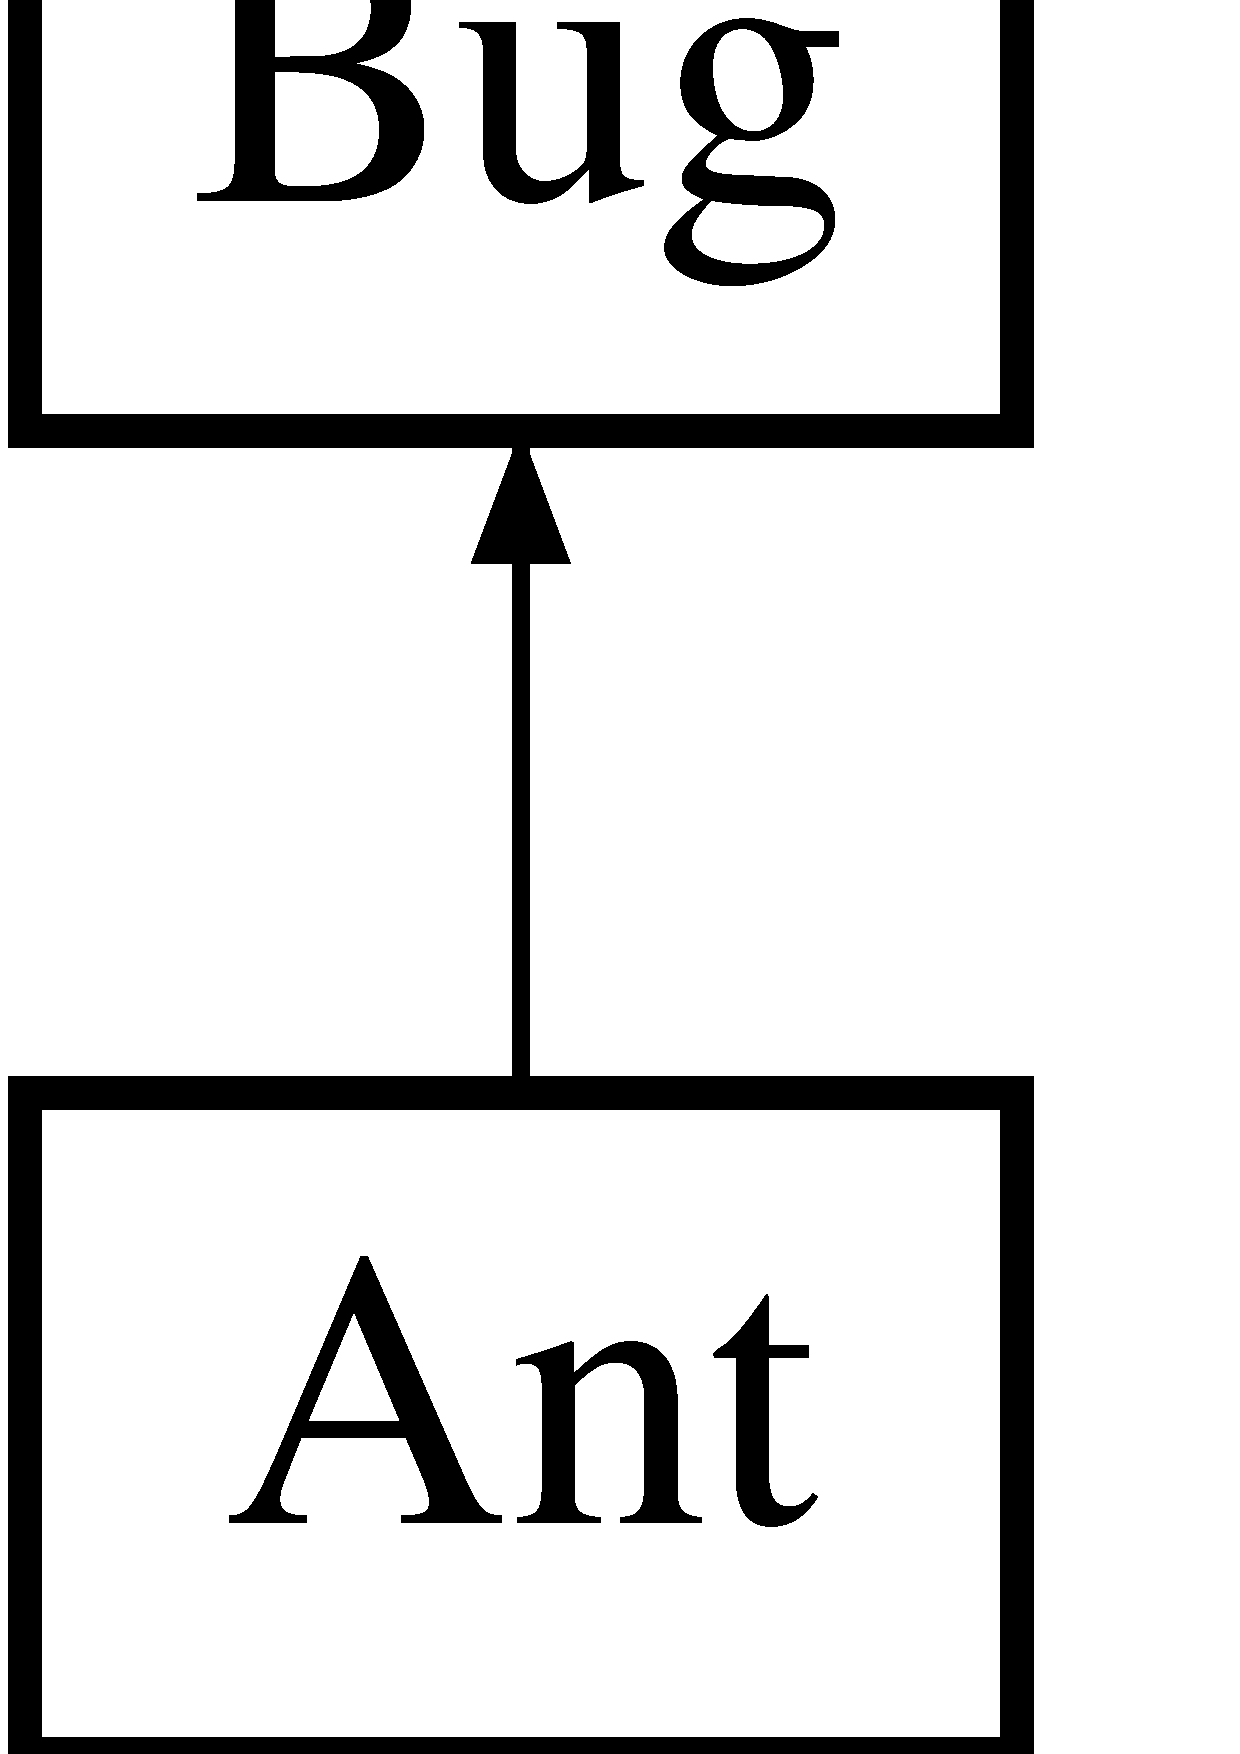
\includegraphics[height=2.000000cm]{classAnt}
\end{center}
\end{figure}
\subsection*{Signaux}
\begin{DoxyCompactItemize}
\item 
void \hyperlink{classBug_ab7379f5a0172e2d536e20f3f29915e02}{dead} (\hyperlink{classBug}{Bug} $\ast$bug)
\begin{DoxyCompactList}\small\item\em Signal de mort de l'insecte. \end{DoxyCompactList}\item 
void \hyperlink{classBug_a33f90dffa55e1dce80dc2416c75a53c8}{goalReached} (\hyperlink{classBug}{Bug} $\ast$bug)
\begin{DoxyCompactList}\small\item\em Signal d'arrivé. \end{DoxyCompactList}\end{DoxyCompactItemize}
\subsection*{Fonctions membres publiques}
\begin{DoxyCompactItemize}
\item 
\hyperlink{classAnt_a52f0aed092463606f4d4edd2091d92eb}{Ant} (double x, double y, double s, double start\_\-angle)
\begin{DoxyCompactList}\small\item\em Constructeur de \hyperlink{classAnt}{Ant}. \end{DoxyCompactList}\item 
\hyperlink{classAnt_a33ca6bd592236726a18a2159908e4116}{$\sim$Ant} ()
\begin{DoxyCompactList}\small\item\em Destructeur de \hyperlink{classAnt}{Ant}. \end{DoxyCompactList}\item 
void \hyperlink{classAnt_abb2b56b817ce45d815251549a77402be}{paint} (QPainter $\ast$painter, const QStyleOptionGraphicsItem $\ast$option, QWidget $\ast$widget)
\begin{DoxyCompactList}\small\item\em Surcharge de la fonction virtuelle pure \hyperlink{classAnt_abb2b56b817ce45d815251549a77402be}{paint()} héritée de QGraphicsObject. \end{DoxyCompactList}\item 
void \hyperlink{classAnt_a64b0e0e7d2605c1a5a0906587ab70920}{hit} (double dmg)
\begin{DoxyCompactList}\small\item\em Infliger des dégats à la fourmi et activer sa capacité spéciale. \end{DoxyCompactList}\item 
QRectF \hyperlink{classBug_a9b39c25361faad07b1bf2dd927d09dab}{boundingRect} () const 
\begin{DoxyCompactList}\small\item\em Surcharge de la fonction boudingRect() hérité de QGraphicsObject. \end{DoxyCompactList}\item 
QPainterPath \hyperlink{classBug_a587a36d3145c2b4dba6c689af22c65ac}{shape} () const 
\begin{DoxyCompactList}\small\item\em Surcharge de la fonction \hyperlink{classBug_a587a36d3145c2b4dba6c689af22c65ac}{shape()} hérité de QGraphicsObject. \end{DoxyCompactList}\item 
short int \hyperlink{classBug_aced471cedcfa855baddf4c827003e755}{getMoveType} ()
\begin{DoxyCompactList}\small\item\em Permet d'accéder à la valeur moveType de l'insecte. \end{DoxyCompactList}\end{DoxyCompactItemize}
\subsection*{Champs de données}
\begin{DoxyCompactItemize}
\item 
\hyperlink{classRender}{Render} $\ast$ \hyperlink{classBug_a7a93aae4e4b7a215c94ff85d0bd6e26d}{parent}
\begin{DoxyCompactList}\small\item\em L'objet \hyperlink{classRender}{Render} parent de l'insecte. \end{DoxyCompactList}\end{DoxyCompactItemize}
\subsection*{Fonctions membres protégées}
\begin{DoxyCompactItemize}
\item 
void \hyperlink{classBug_a8e0ea03e85c9324a13328da60e5c52ee}{advance} (int step)
\begin{DoxyCompactList}\small\item\em Implémentation de la fonction virtuelle pure \hyperlink{classBug_a8e0ea03e85c9324a13328da60e5c52ee}{advance()} héritée de QGGaphicsObject. \end{DoxyCompactList}\end{DoxyCompactItemize}
\subsection*{Attributs protégés}
\begin{DoxyCompactItemize}
\item 
double \hyperlink{classBug_a27a0f0b84d15525e409955509e6e3c42}{size}
\begin{DoxyCompactList}\small\item\em Taille. \end{DoxyCompactList}\item 
int \hyperlink{classBug_ad7e3597cf049f1051be94fcaf2fd3598}{frame}
\begin{DoxyCompactList}\small\item\em Compteur de frame. \end{DoxyCompactList}\item 
double \hyperlink{classBug_a13b95fbf23748ea853b01bfd0b0e7fc8}{speed}
\begin{DoxyCompactList}\small\item\em Vitesse de base. \end{DoxyCompactList}\end{DoxyCompactItemize}
\subsection*{Connecteurs privés}
\begin{DoxyCompactItemize}
\item 
\hypertarget{classAnt_a1261f3d930faf4c98f06e173203a3d72}{
void \hyperlink{classAnt_a1261f3d930faf4c98f06e173203a3d72}{slowDown} ()}
\label{classAnt_a1261f3d930faf4c98f06e173203a3d72}

\begin{DoxyCompactList}\small\item\em Slot appelé pour ralentir la fourmi Après 5 secondes, le timer émet un signal timeout qui appelle la fonction \hyperlink{classAnt_a1261f3d930faf4c98f06e173203a3d72}{slowDown()} de la fourmi pour reprendre sa vitesse initiale? \end{DoxyCompactList}\end{DoxyCompactItemize}
\subsection*{Attributs privés}
\begin{DoxyCompactItemize}
\item 
QImage $\ast$ \hyperlink{classAnt_af7d498fe6677833f371d3d9561727678}{image} \mbox{[}3\mbox{]}
\begin{DoxyCompactList}\small\item\em Cache d'images. \end{DoxyCompactList}\item 
QTimer $\ast$ \hyperlink{classAnt_a0535768a0f4cb7682a13c6cd514cf7b0}{timer}
\begin{DoxyCompactList}\small\item\em Timer de ralentissement. \end{DoxyCompactList}\end{DoxyCompactItemize}


\subsection{Description détaillée}
Définie les caractéristiques spécifiques aux fourmis, comme leur graphisme, leur type de déplacement (FLY ou CRAWL)... 

\subsection{Documentation des constructeurs et destructeur}
\hypertarget{classAnt_a52f0aed092463606f4d4edd2091d92eb}{
\index{Ant@{Ant}!Ant@{Ant}}
\index{Ant@{Ant}!Ant@{Ant}}
\subsubsection[{Ant}]{\setlength{\rightskip}{0pt plus 5cm}Ant::Ant (
\begin{DoxyParamCaption}
\item[{double}]{x, }
\item[{double}]{y, }
\item[{double}]{s, }
\item[{double}]{start\_\-angle}
\end{DoxyParamCaption}
)}}
\label{classAnt_a52f0aed092463606f4d4edd2091d92eb}
Ce constructeur initialise les images en cache de la fourmi et appelle le constructeur parent (\hyperlink{classBug}{Bug}) avec les bons paramètres correspondant aux caractéristique d'une fourmi. 
\begin{DoxyParams}{Paramètres}
{\em x} & Un double correspondant à l'abscisse du point de départ des insectes. \\
\hline
{\em y} & Un double correspondant à l'ordonnée du point de départ des insectes. \\
\hline
{\em s} & La taille de la fourmi, influe sur la taille de la représentation graphiques et sur ses autres caractéristiques. \\
\hline
{\em start\_\-angle} & L'angle vers lequel fait face le départ des insectes. \\
\hline
\end{DoxyParams}
\hypertarget{classAnt_a33ca6bd592236726a18a2159908e4116}{
\index{Ant@{Ant}!$\sim$Ant@{$\sim$Ant}}
\index{$\sim$Ant@{$\sim$Ant}!Ant@{Ant}}
\subsubsection[{$\sim$Ant}]{\setlength{\rightskip}{0pt plus 5cm}Ant::$\sim$Ant (
\begin{DoxyParamCaption}
{}
\end{DoxyParamCaption}
)}}
\label{classAnt_a33ca6bd592236726a18a2159908e4116}
Désalloue la mémoire des images de la fourmi en cache. 

\subsection{Documentation des fonctions membres}
\hypertarget{classBug_a8e0ea03e85c9324a13328da60e5c52ee}{
\index{Ant@{Ant}!advance@{advance}}
\index{advance@{advance}!Ant@{Ant}}
\subsubsection[{advance}]{\setlength{\rightskip}{0pt plus 5cm}void Bug::advance (
\begin{DoxyParamCaption}
\item[{int}]{step}
\end{DoxyParamCaption}
)\hspace{0.3cm}{\ttfamily  \mbox{[}protected, inherited\mbox{]}}}}
\label{classBug_a8e0ea03e85c9324a13328da60e5c52ee}
Implémentation de la fonction virtuelle pure \hyperlink{classBug_a8e0ea03e85c9324a13328da60e5c52ee}{advance()} héritée de QGGaphicsObject. 
\begin{DoxyParams}{Paramètres}
{\em step} & La fonction est appelé deux fois automatiquement par QT à chaque update(), une fois avec 0 comme paramètre puis une fois avec 1. \\
\hline
\end{DoxyParams}
\hypertarget{classBug_a9b39c25361faad07b1bf2dd927d09dab}{
\index{Ant@{Ant}!boundingRect@{boundingRect}}
\index{boundingRect@{boundingRect}!Ant@{Ant}}
\subsubsection[{boundingRect}]{\setlength{\rightskip}{0pt plus 5cm}QRectF Bug::boundingRect (
\begin{DoxyParamCaption}
{}
\end{DoxyParamCaption}
) const\hspace{0.3cm}{\ttfamily  \mbox{[}inherited\mbox{]}}}}
\label{classBug_a9b39c25361faad07b1bf2dd927d09dab}
Fonction appelé automatiquement par QT pour savoir s'il doit ou non réafficher l'insecte. \begin{DoxyReturn}{Renvoie}
Un objet QRectF correspondant au rectangle englobant l'ensemble du dessin de l'insecte. 
\end{DoxyReturn}
\hypertarget{classBug_ab7379f5a0172e2d536e20f3f29915e02}{
\index{Ant@{Ant}!dead@{dead}}
\index{dead@{dead}!Ant@{Ant}}
\subsubsection[{dead}]{\setlength{\rightskip}{0pt plus 5cm}void Bug::dead (
\begin{DoxyParamCaption}
\item[{{\bf Bug} $\ast$}]{bug}
\end{DoxyParamCaption}
)\hspace{0.3cm}{\ttfamily  \mbox{[}signal, inherited\mbox{]}}}}
\label{classBug_ab7379f5a0172e2d536e20f3f29915e02}
Signal émit lorsque l'insecte est tué. 
\begin{DoxyParams}{Paramètres}
{\em bug} & Un pointeur vers l'insecte qui vient de mourir. \\
\hline
\end{DoxyParams}
\hypertarget{classBug_aced471cedcfa855baddf4c827003e755}{
\index{Ant@{Ant}!getMoveType@{getMoveType}}
\index{getMoveType@{getMoveType}!Ant@{Ant}}
\subsubsection[{getMoveType}]{\setlength{\rightskip}{0pt plus 5cm}short int Bug::getMoveType (
\begin{DoxyParamCaption}
{}
\end{DoxyParamCaption}
)\hspace{0.3cm}{\ttfamily  \mbox{[}inherited\mbox{]}}}}
\label{classBug_aced471cedcfa855baddf4c827003e755}
\begin{DoxyReturn}{Renvoie}
la valeur prédéfinie FLY ou CRAWL. 
\end{DoxyReturn}
\hypertarget{classBug_a33f90dffa55e1dce80dc2416c75a53c8}{
\index{Ant@{Ant}!goalReached@{goalReached}}
\index{goalReached@{goalReached}!Ant@{Ant}}
\subsubsection[{goalReached}]{\setlength{\rightskip}{0pt plus 5cm}void Bug::goalReached (
\begin{DoxyParamCaption}
\item[{{\bf Bug} $\ast$}]{bug}
\end{DoxyParamCaption}
)\hspace{0.3cm}{\ttfamily  \mbox{[}signal, inherited\mbox{]}}}}
\label{classBug_a33f90dffa55e1dce80dc2416c75a53c8}
Signal émit par l'insecte lorsqu'il atteint son but. 
\begin{DoxyParams}{Paramètres}
{\em bug} & Un pointeur vers l'insecte. \\
\hline
\end{DoxyParams}
\hypertarget{classAnt_a64b0e0e7d2605c1a5a0906587ab70920}{
\index{Ant@{Ant}!hit@{hit}}
\index{hit@{hit}!Ant@{Ant}}
\subsubsection[{hit}]{\setlength{\rightskip}{0pt plus 5cm}void Ant::hit (
\begin{DoxyParamCaption}
\item[{double}]{dmg}
\end{DoxyParamCaption}
)}}
\label{classAnt_a64b0e0e7d2605c1a5a0906587ab70920}
Appelle la méthode \hyperlink{classBug_a63402c05b5ba3fb034e41f1ced0e4b9f}{Bug::hit()} pour infliger les dégats, et lance le timer pour accélérer la fourmi pendant 5 secondes. 
\begin{DoxyParams}{Paramètres}
{\em dmg} & Un double correspondant au montant de dégats à infliger avec réduction. \\
\hline
\end{DoxyParams}


Réimplémentée à partir de \hyperlink{classBug_a63402c05b5ba3fb034e41f1ced0e4b9f}{Bug}.

\hypertarget{classAnt_abb2b56b817ce45d815251549a77402be}{
\index{Ant@{Ant}!paint@{paint}}
\index{paint@{paint}!Ant@{Ant}}
\subsubsection[{paint}]{\setlength{\rightskip}{0pt plus 5cm}void Ant::paint (
\begin{DoxyParamCaption}
\item[{QPainter $\ast$}]{painter, }
\item[{const QStyleOptionGraphicsItem $\ast$}]{option, }
\item[{QWidget $\ast$}]{widget}
\end{DoxyParamCaption}
)}}
\label{classAnt_abb2b56b817ce45d815251549a77402be}
Est appelé automatiquement par Qt pour redessiner la fourmi. \hypertarget{classBug_a587a36d3145c2b4dba6c689af22c65ac}{
\index{Ant@{Ant}!shape@{shape}}
\index{shape@{shape}!Ant@{Ant}}
\subsubsection[{shape}]{\setlength{\rightskip}{0pt plus 5cm}QPainterPath Bug::shape (
\begin{DoxyParamCaption}
{}
\end{DoxyParamCaption}
) const\hspace{0.3cm}{\ttfamily  \mbox{[}inherited\mbox{]}}}}
\label{classBug_a587a36d3145c2b4dba6c689af22c65ac}
Fonction utilisé par QT pour traiter les collisions entre objets graphiques. \begin{DoxyReturn}{Renvoie}
Un object QPainterPath correspondant au contour de collision de l'insecte. 
\end{DoxyReturn}


\subsection{Documentation des champs}
\hypertarget{classBug_ad7e3597cf049f1051be94fcaf2fd3598}{
\index{Ant@{Ant}!frame@{frame}}
\index{frame@{frame}!Ant@{Ant}}
\subsubsection[{frame}]{\setlength{\rightskip}{0pt plus 5cm}int {\bf Bug::frame}\hspace{0.3cm}{\ttfamily  \mbox{[}protected, inherited\mbox{]}}}}
\label{classBug_ad7e3597cf049f1051be94fcaf2fd3598}
Compteur d'image utilisé pour afficher successivement chaque image des animations. \hypertarget{classAnt_af7d498fe6677833f371d3d9561727678}{
\index{Ant@{Ant}!image@{image}}
\index{image@{image}!Ant@{Ant}}
\subsubsection[{image}]{\setlength{\rightskip}{0pt plus 5cm}QImage$\ast$ {\bf Ant::image}\mbox{[}3\mbox{]}\hspace{0.3cm}{\ttfamily  \mbox{[}private\mbox{]}}}}
\label{classAnt_af7d498fe6677833f371d3d9561727678}
Les images de la fourmis à chaque position, redimensionnées en fonction de sa taille et mises en cache pour un affichage plus rapide. \hypertarget{classBug_a7a93aae4e4b7a215c94ff85d0bd6e26d}{
\index{Ant@{Ant}!parent@{parent}}
\index{parent@{parent}!Ant@{Ant}}
\subsubsection[{parent}]{\setlength{\rightskip}{0pt plus 5cm}{\bf Render}$\ast$ {\bf Bug::parent}\hspace{0.3cm}{\ttfamily  \mbox{[}inherited\mbox{]}}}}
\label{classBug_a7a93aae4e4b7a215c94ff85d0bd6e26d}
Quand on ajoute un insecte à l'objet \hyperlink{classRender}{Render} par la méthode addBug(), cet attribut est automatiquement initialisé. \hypertarget{classBug_a27a0f0b84d15525e409955509e6e3c42}{
\index{Ant@{Ant}!size@{size}}
\index{size@{size}!Ant@{Ant}}
\subsubsection[{size}]{\setlength{\rightskip}{0pt plus 5cm}double {\bf Bug::size}\hspace{0.3cm}{\ttfamily  \mbox{[}protected, inherited\mbox{]}}}}
\label{classBug_a27a0f0b84d15525e409955509e6e3c42}
La taille de l'insecte, influe à la fois sur la taille de la représentation graphique et sur les caractéristiques de l'insecte.' \hypertarget{classBug_a13b95fbf23748ea853b01bfd0b0e7fc8}{
\index{Ant@{Ant}!speed@{speed}}
\index{speed@{speed}!Ant@{Ant}}
\subsubsection[{speed}]{\setlength{\rightskip}{0pt plus 5cm}double {\bf Bug::speed}\hspace{0.3cm}{\ttfamily  \mbox{[}protected, inherited\mbox{]}}}}
\label{classBug_a13b95fbf23748ea853b01bfd0b0e7fc8}
La vitesse en case/seconde à laquelle se déplace l'insecte. \hypertarget{classAnt_a0535768a0f4cb7682a13c6cd514cf7b0}{
\index{Ant@{Ant}!timer@{timer}}
\index{timer@{timer}!Ant@{Ant}}
\subsubsection[{timer}]{\setlength{\rightskip}{0pt plus 5cm}QTimer$\ast$ {\bf Ant::timer}\hspace{0.3cm}{\ttfamily  \mbox{[}private\mbox{]}}}}
\label{classAnt_a0535768a0f4cb7682a13c6cd514cf7b0}
Quand une fourmis est blessée, elle accélère pendant 5 secondes, ce timer permet de faire ce décompte. 

La documentation de cette classe a été générée à partir des fichiers suivants :\begin{DoxyCompactItemize}
\item 
src/Ant.h\item 
src/Ant.cpp\end{DoxyCompactItemize}

\hypertarget{classBug}{
\section{Référence de la classe Bug}
\label{classBug}\index{Bug@{Bug}}
}


Classe abstraite dont héritent les ennemis.  




{\ttfamily \#include $<$Bug.h$>$}

Graphe d'héritage de Bug:\begin{figure}[H]
\begin{center}
\leavevmode
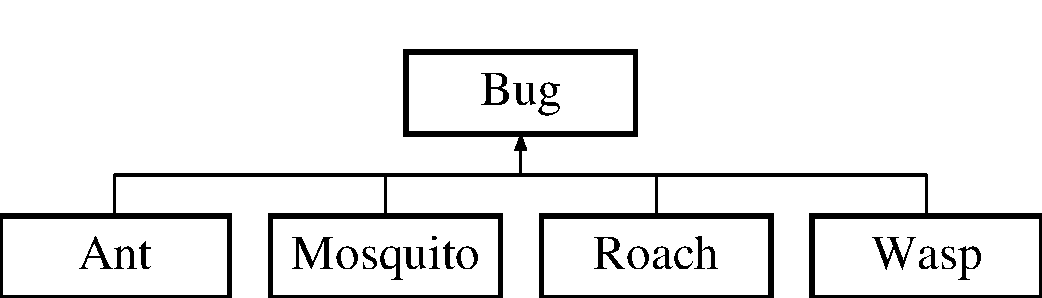
\includegraphics[height=2.000000cm]{classBug}
\end{center}
\end{figure}
\subsection*{Signaux}
\begin{DoxyCompactItemize}
\item 
void \hyperlink{classBug_ab7379f5a0172e2d536e20f3f29915e02}{dead} (\hyperlink{classBug}{Bug} $\ast$bug)
\begin{DoxyCompactList}\small\item\em Signal de mort de l'insecte. \end{DoxyCompactList}\item 
void \hyperlink{classBug_a33f90dffa55e1dce80dc2416c75a53c8}{goalReached} (\hyperlink{classBug}{Bug} $\ast$bug)
\begin{DoxyCompactList}\small\item\em Signal d'arrivé. \end{DoxyCompactList}\end{DoxyCompactItemize}
\subsection*{Fonctions membres publiques}
\begin{DoxyCompactItemize}
\item 
\hyperlink{classBug_a1d3140d50abd44257d5e0b1b6dcb4514}{Bug} (double x, double y, double s, double health, double res, double start\_\-angle, double init\_\-speed, short int type)
\begin{DoxyCompactList}\small\item\em Constructeur de \hyperlink{classBug}{Bug}. \end{DoxyCompactList}\item 
QRectF \hyperlink{classBug_a9b39c25361faad07b1bf2dd927d09dab}{boundingRect} () const 
\begin{DoxyCompactList}\small\item\em Surcharge de la fonction boudingRect() hérité de QGraphicsObject. \end{DoxyCompactList}\item 
QPainterPath \hyperlink{classBug_a587a36d3145c2b4dba6c689af22c65ac}{shape} () const 
\begin{DoxyCompactList}\small\item\em Surcharge de la fonction \hyperlink{classBug_a587a36d3145c2b4dba6c689af22c65ac}{shape()} hérité de QGraphicsObject. \end{DoxyCompactList}\item 
void \hyperlink{classBug_a63402c05b5ba3fb034e41f1ced0e4b9f}{hit} (double dmg)
\begin{DoxyCompactList}\small\item\em Infliger des dégats à l'insecte. \end{DoxyCompactList}\item 
short int \hyperlink{classBug_aced471cedcfa855baddf4c827003e755}{getMoveType} ()
\begin{DoxyCompactList}\small\item\em Permet d'accéder à la valeur moveType de l'insecte. \end{DoxyCompactList}\end{DoxyCompactItemize}
\subsection*{Champs de données}
\begin{DoxyCompactItemize}
\item 
\hyperlink{classRender}{Render} $\ast$ \hyperlink{classBug_a7a93aae4e4b7a215c94ff85d0bd6e26d}{parent}
\begin{DoxyCompactList}\small\item\em L'objet \hyperlink{classRender}{Render} parent de l'insecte. \end{DoxyCompactList}\end{DoxyCompactItemize}
\subsection*{Fonctions membres protégées}
\begin{DoxyCompactItemize}
\item 
void \hyperlink{classBug_a8e0ea03e85c9324a13328da60e5c52ee}{advance} (int step)
\begin{DoxyCompactList}\small\item\em Implémentation de la fonction virtuelle pure \hyperlink{classBug_a8e0ea03e85c9324a13328da60e5c52ee}{advance()} héritée de QGGaphicsObject. \end{DoxyCompactList}\end{DoxyCompactItemize}
\subsection*{Attributs protégés}
\begin{DoxyCompactItemize}
\item 
double \hyperlink{classBug_a27a0f0b84d15525e409955509e6e3c42}{size}
\begin{DoxyCompactList}\small\item\em Taille. \end{DoxyCompactList}\item 
int \hyperlink{classBug_ad7e3597cf049f1051be94fcaf2fd3598}{frame}
\begin{DoxyCompactList}\small\item\em Compteur de frame. \end{DoxyCompactList}\item 
double \hyperlink{classBug_a13b95fbf23748ea853b01bfd0b0e7fc8}{speed}
\begin{DoxyCompactList}\small\item\em Vitesse de base. \end{DoxyCompactList}\end{DoxyCompactItemize}
\subsection*{Attributs privés}
\begin{DoxyCompactItemize}
\item 
double \hyperlink{classBug_a3ebb13469010dbcd7bd7875455e022c3}{hp}
\begin{DoxyCompactList}\small\item\em Point de vie. \end{DoxyCompactList}\item 
double \hyperlink{classBug_a98590009992312ec6508e334bd02e529}{resist}
\begin{DoxyCompactList}\small\item\em Résistance. \end{DoxyCompactList}\item 
double \hyperlink{classBug_a096a8babe1be6df06b5dea87dc3eb1fe}{angle}
\begin{DoxyCompactList}\small\item\em Angle des déplacements. \end{DoxyCompactList}\item 
short int \hyperlink{classBug_a00484a34d1e537e92b0bba7e2e5ddbeb}{moveType}
\begin{DoxyCompactList}\small\item\em Type de déplacement. \end{DoxyCompactList}\item 
QPoint \hyperlink{classBug_aead6b14a5cfd6713e8913f3e84cd6797}{lastSquare}
\begin{DoxyCompactList}\small\item\em Case d'origine. \end{DoxyCompactList}\end{DoxyCompactItemize}


\subsection{Description détaillée}
Cette classe définie les actions de base commune à tous les insectes (l'affichage, la vie et les déplacements entre autres). 

\subsection{Documentation des constructeurs et destructeur}
\hypertarget{classBug_a1d3140d50abd44257d5e0b1b6dcb4514}{
\index{Bug@{Bug}!Bug@{Bug}}
\index{Bug@{Bug}!Bug@{Bug}}
\subsubsection[{Bug}]{\setlength{\rightskip}{0pt plus 5cm}Bug::Bug (
\begin{DoxyParamCaption}
\item[{double}]{x, }
\item[{double}]{y, }
\item[{double}]{s, }
\item[{double}]{health, }
\item[{double}]{res, }
\item[{double}]{start\_\-angle, }
\item[{double}]{init\_\-speed, }
\item[{short int}]{type}
\end{DoxyParamCaption}
)}}
\label{classBug_a1d3140d50abd44257d5e0b1b6dcb4514}
La classe \hyperlink{classBug}{Bug} étant abstraite, le constructeur sera toujours appelé par ses classes filles (\hyperlink{classWasp}{Wasp}, \hyperlink{classAnt}{Ant}, \hyperlink{classMosquito}{Mosquito}, \hyperlink{classRoach}{Roach}) avec les bons paramètres. 
\begin{DoxyParams}{Paramètres}
{\em x} & Un double correspondant à l'abscisse du point de départ des insectes. \\
\hline
{\em y} & Un double correspondant à l'ordonnée du point de départ des insectes. \\
\hline
{\em s} & La taille de l'insecte à créer. \\
\hline
{\em health} & Un double donnant la vitalité initiale de l'insecte. \\
\hline
{\em res} & Un double donnant la résistance aux dégats de l'insecte. \\
\hline
{\em start\_\-angle} & L'angle vers lequel fait face le départ des insectes. \\
\hline
{\em init\_\-speed} & La vitesse initiale de l'insecte. \\
\hline
{\em type} & Prends une des valeurs prédéfinies FLY ou CRAWL correspondant au type de déplacement de l'insecte. \\
\hline
\end{DoxyParams}


\subsection{Documentation des fonctions membres}
\hypertarget{classBug_a8e0ea03e85c9324a13328da60e5c52ee}{
\index{Bug@{Bug}!advance@{advance}}
\index{advance@{advance}!Bug@{Bug}}
\subsubsection[{advance}]{\setlength{\rightskip}{0pt plus 5cm}void Bug::advance (
\begin{DoxyParamCaption}
\item[{int}]{step}
\end{DoxyParamCaption}
)\hspace{0.3cm}{\ttfamily  \mbox{[}protected\mbox{]}}}}
\label{classBug_a8e0ea03e85c9324a13328da60e5c52ee}
Implémentation de la fonction virtuelle pure \hyperlink{classBug_a8e0ea03e85c9324a13328da60e5c52ee}{advance()} héritée de QGGaphicsObject. 
\begin{DoxyParams}{Paramètres}
{\em step} & La fonction est appelé deux fois automatiquement par QT à chaque update(), une fois avec 0 comme paramètre puis une fois avec 1. \\
\hline
\end{DoxyParams}
\hypertarget{classBug_a9b39c25361faad07b1bf2dd927d09dab}{
\index{Bug@{Bug}!boundingRect@{boundingRect}}
\index{boundingRect@{boundingRect}!Bug@{Bug}}
\subsubsection[{boundingRect}]{\setlength{\rightskip}{0pt plus 5cm}QRectF Bug::boundingRect (
\begin{DoxyParamCaption}
{}
\end{DoxyParamCaption}
) const}}
\label{classBug_a9b39c25361faad07b1bf2dd927d09dab}
Fonction appelé automatiquement par QT pour savoir s'il doit ou non réafficher l'insecte. \begin{DoxyReturn}{Renvoie}
Un objet QRectF correspondant au rectangle englobant l'ensemble du dessin de l'insecte. 
\end{DoxyReturn}
\hypertarget{classBug_ab7379f5a0172e2d536e20f3f29915e02}{
\index{Bug@{Bug}!dead@{dead}}
\index{dead@{dead}!Bug@{Bug}}
\subsubsection[{dead}]{\setlength{\rightskip}{0pt plus 5cm}void Bug::dead (
\begin{DoxyParamCaption}
\item[{{\bf Bug} $\ast$}]{bug}
\end{DoxyParamCaption}
)\hspace{0.3cm}{\ttfamily  \mbox{[}signal\mbox{]}}}}
\label{classBug_ab7379f5a0172e2d536e20f3f29915e02}
Signal émit lorsque l'insecte est tué. 
\begin{DoxyParams}{Paramètres}
{\em bug} & Un pointeur vers l'insecte qui vient de mourir. \\
\hline
\end{DoxyParams}
\hypertarget{classBug_aced471cedcfa855baddf4c827003e755}{
\index{Bug@{Bug}!getMoveType@{getMoveType}}
\index{getMoveType@{getMoveType}!Bug@{Bug}}
\subsubsection[{getMoveType}]{\setlength{\rightskip}{0pt plus 5cm}short int Bug::getMoveType (
\begin{DoxyParamCaption}
{}
\end{DoxyParamCaption}
)}}
\label{classBug_aced471cedcfa855baddf4c827003e755}
\begin{DoxyReturn}{Renvoie}
la valeur prédéfinie FLY ou CRAWL. 
\end{DoxyReturn}
\hypertarget{classBug_a33f90dffa55e1dce80dc2416c75a53c8}{
\index{Bug@{Bug}!goalReached@{goalReached}}
\index{goalReached@{goalReached}!Bug@{Bug}}
\subsubsection[{goalReached}]{\setlength{\rightskip}{0pt plus 5cm}void Bug::goalReached (
\begin{DoxyParamCaption}
\item[{{\bf Bug} $\ast$}]{bug}
\end{DoxyParamCaption}
)\hspace{0.3cm}{\ttfamily  \mbox{[}signal\mbox{]}}}}
\label{classBug_a33f90dffa55e1dce80dc2416c75a53c8}
Signal émit par l'insecte lorsqu'il atteint son but. 
\begin{DoxyParams}{Paramètres}
{\em bug} & Un pointeur vers l'insecte. \\
\hline
\end{DoxyParams}
\hypertarget{classBug_a63402c05b5ba3fb034e41f1ced0e4b9f}{
\index{Bug@{Bug}!hit@{hit}}
\index{hit@{hit}!Bug@{Bug}}
\subsubsection[{hit}]{\setlength{\rightskip}{0pt plus 5cm}void Bug::hit (
\begin{DoxyParamCaption}
\item[{double}]{dmg}
\end{DoxyParamCaption}
)}}
\label{classBug_a63402c05b5ba3fb034e41f1ced0e4b9f}
Fonction pouvant être appelée pour infliger des dégats à l'insecte (par exemple par les projectiles des tours). 
\begin{DoxyParams}{Paramètres}
{\em dmg} & Un double correspondant au point de dégat à infliger (avant réduction par la résistance de l'insecte). \\
\hline
\end{DoxyParams}


Réimplémentée dans \hyperlink{classAnt_a64b0e0e7d2605c1a5a0906587ab70920}{Ant}.

\hypertarget{classBug_a587a36d3145c2b4dba6c689af22c65ac}{
\index{Bug@{Bug}!shape@{shape}}
\index{shape@{shape}!Bug@{Bug}}
\subsubsection[{shape}]{\setlength{\rightskip}{0pt plus 5cm}QPainterPath Bug::shape (
\begin{DoxyParamCaption}
{}
\end{DoxyParamCaption}
) const}}
\label{classBug_a587a36d3145c2b4dba6c689af22c65ac}
Fonction utilisé par QT pour traiter les collisions entre objets graphiques. \begin{DoxyReturn}{Renvoie}
Un object QPainterPath correspondant au contour de collision de l'insecte. 
\end{DoxyReturn}


\subsection{Documentation des champs}
\hypertarget{classBug_a096a8babe1be6df06b5dea87dc3eb1fe}{
\index{Bug@{Bug}!angle@{angle}}
\index{angle@{angle}!Bug@{Bug}}
\subsubsection[{angle}]{\setlength{\rightskip}{0pt plus 5cm}double {\bf Bug::angle}\hspace{0.3cm}{\ttfamily  \mbox{[}private\mbox{]}}}}
\label{classBug_a096a8babe1be6df06b5dea87dc3eb1fe}
Angle dans lequel l'insecte se déplace. \hypertarget{classBug_ad7e3597cf049f1051be94fcaf2fd3598}{
\index{Bug@{Bug}!frame@{frame}}
\index{frame@{frame}!Bug@{Bug}}
\subsubsection[{frame}]{\setlength{\rightskip}{0pt plus 5cm}int {\bf Bug::frame}\hspace{0.3cm}{\ttfamily  \mbox{[}protected\mbox{]}}}}
\label{classBug_ad7e3597cf049f1051be94fcaf2fd3598}
Compteur d'image utilisé pour afficher successivement chaque image des animations. \hypertarget{classBug_a3ebb13469010dbcd7bd7875455e022c3}{
\index{Bug@{Bug}!hp@{hp}}
\index{hp@{hp}!Bug@{Bug}}
\subsubsection[{hp}]{\setlength{\rightskip}{0pt plus 5cm}double {\bf Bug::hp}\hspace{0.3cm}{\ttfamily  \mbox{[}private\mbox{]}}}}
\label{classBug_a3ebb13469010dbcd7bd7875455e022c3}
La vitalité de l'insecte, quand elle atteint 0, l'insecte meurt et le joueur gagne 1 crédit. \hypertarget{classBug_aead6b14a5cfd6713e8913f3e84cd6797}{
\index{Bug@{Bug}!lastSquare@{lastSquare}}
\index{lastSquare@{lastSquare}!Bug@{Bug}}
\subsubsection[{lastSquare}]{\setlength{\rightskip}{0pt plus 5cm}QPoint {\bf Bug::lastSquare}\hspace{0.3cm}{\ttfamily  \mbox{[}private\mbox{]}}}}
\label{classBug_aead6b14a5cfd6713e8913f3e84cd6797}
Dernière case visité par l'insecte. Elle est utilisé dans la détection de changement de case. \hypertarget{classBug_a00484a34d1e537e92b0bba7e2e5ddbeb}{
\index{Bug@{Bug}!moveType@{moveType}}
\index{moveType@{moveType}!Bug@{Bug}}
\subsubsection[{moveType}]{\setlength{\rightskip}{0pt plus 5cm}short int {\bf Bug::moveType}\hspace{0.3cm}{\ttfamily  \mbox{[}private\mbox{]}}}}
\label{classBug_a00484a34d1e537e92b0bba7e2e5ddbeb}
Peut prendre les valeurs prédéfinies FLY ou CRAWL. \hypertarget{classBug_a7a93aae4e4b7a215c94ff85d0bd6e26d}{
\index{Bug@{Bug}!parent@{parent}}
\index{parent@{parent}!Bug@{Bug}}
\subsubsection[{parent}]{\setlength{\rightskip}{0pt plus 5cm}{\bf Render}$\ast$ {\bf Bug::parent}}}
\label{classBug_a7a93aae4e4b7a215c94ff85d0bd6e26d}
Quand on ajoute un insecte à l'objet \hyperlink{classRender}{Render} par la méthode addBug(), cet attribut est automatiquement initialisé. \hypertarget{classBug_a98590009992312ec6508e334bd02e529}{
\index{Bug@{Bug}!resist@{resist}}
\index{resist@{resist}!Bug@{Bug}}
\subsubsection[{resist}]{\setlength{\rightskip}{0pt plus 5cm}double {\bf Bug::resist}\hspace{0.3cm}{\ttfamily  \mbox{[}private\mbox{]}}}}
\label{classBug_a98590009992312ec6508e334bd02e529}
La résistance aux dégats de l'insecte. \hypertarget{classBug_a27a0f0b84d15525e409955509e6e3c42}{
\index{Bug@{Bug}!size@{size}}
\index{size@{size}!Bug@{Bug}}
\subsubsection[{size}]{\setlength{\rightskip}{0pt plus 5cm}double {\bf Bug::size}\hspace{0.3cm}{\ttfamily  \mbox{[}protected\mbox{]}}}}
\label{classBug_a27a0f0b84d15525e409955509e6e3c42}
La taille de l'insecte, influe à la fois sur la taille de la représentation graphique et sur les caractéristiques de l'insecte.' \hypertarget{classBug_a13b95fbf23748ea853b01bfd0b0e7fc8}{
\index{Bug@{Bug}!speed@{speed}}
\index{speed@{speed}!Bug@{Bug}}
\subsubsection[{speed}]{\setlength{\rightskip}{0pt plus 5cm}double {\bf Bug::speed}\hspace{0.3cm}{\ttfamily  \mbox{[}protected\mbox{]}}}}
\label{classBug_a13b95fbf23748ea853b01bfd0b0e7fc8}
La vitesse en case/seconde à laquelle se déplace l'insecte. 

La documentation de cette classe a été générée à partir des fichiers suivants :\begin{DoxyCompactItemize}
\item 
src/Bug.h\item 
src/Bug.cpp\item 
src/moc\_\-Bug.cpp\end{DoxyCompactItemize}

\hypertarget{classHatchery}{
\section{Référence de la classe Hatchery}
\label{classHatchery}\index{Hatchery@{Hatchery}}
}


Classe implémentation du design pattern Factory.  




{\ttfamily \#include $<$Hatchery.h$>$}

\subsection*{Fonctions membres publiques}
\begin{DoxyCompactItemize}
\item 
\hyperlink{classHatchery_a8e86b7578b70f37fb3f7ed2e69c765b7}{Hatchery} (double start\_\-x, double start\_\-y, double start\_\-angle)
\begin{DoxyCompactList}\small\item\em Constructeur d'Hatchery. \end{DoxyCompactList}\item 
\hyperlink{classBug}{Bug} $\ast$ \hyperlink{classHatchery_af90645b2be3e8890829a69347846a934}{spawnBug} (QString race, double size)
\begin{DoxyCompactList}\small\item\em Crée un nouvel insecte de la race et de la taille données. \end{DoxyCompactList}\item 
\hyperlink{classBug}{Bug} $\ast$ \hyperlink{classHatchery_ad062be27d539081dd061eec1898df12b}{spawnBug} (QString race, double size, QPointF pos, double spawn\_\-angle)
\begin{DoxyCompactList}\small\item\em Crée un nouvel insecte de la race et de la taille données. \end{DoxyCompactList}\end{DoxyCompactItemize}
\subsection*{Attributs privés}
\begin{DoxyCompactItemize}
\item 
double \hyperlink{classHatchery_ae56bf748a2046b42e2b174c17e4caeda}{x}
\begin{DoxyCompactList}\small\item\em Abscisse du spawn des insectes. \end{DoxyCompactList}\item 
double \hyperlink{classHatchery_a99f0ef4a290d0bc1e65976b5979b29b7}{y}
\begin{DoxyCompactList}\small\item\em Ordonnée du spawn des insectes. \end{DoxyCompactList}\item 
double \hyperlink{classHatchery_a4e56c9314b9a9dfe1718d43e30f3d4d0}{angle}
\begin{DoxyCompactList}\small\item\em Angle vers lequel fait face le spawn des insectes. \end{DoxyCompactList}\end{DoxyCompactItemize}


\subsection{Description détaillée}
Design pattern Factory utilisé pour créer un nouvel insecte au niveau du spawn. 

\subsection{Documentation des constructeurs et destructeur}
\hypertarget{classHatchery_a8e86b7578b70f37fb3f7ed2e69c765b7}{
\index{Hatchery@{Hatchery}!Hatchery@{Hatchery}}
\index{Hatchery@{Hatchery}!Hatchery@{Hatchery}}
\subsubsection[{Hatchery}]{\setlength{\rightskip}{0pt plus 5cm}Hatchery::Hatchery (
\begin{DoxyParamCaption}
\item[{double}]{start\_\-x, }
\item[{double}]{start\_\-y, }
\item[{double}]{start\_\-angle}
\end{DoxyParamCaption}
)}}
\label{classHatchery_a8e86b7578b70f37fb3f7ed2e69c765b7}
Permet d'instancier un objet \hyperlink{classHatchery}{Hatchery} pour initialiser la position et l'angle du spawn des insectes. 
\begin{DoxyParams}{Paramètres}
{\em start\_\-x} & Un double correspondant à l'abscisse du point de départ des insectes. \\
\hline
{\em start\_\-y} & Un double correspondant à l'ordonnée du point de départ des insectes. \\
\hline
{\em start\_\-angle} & Un double correspondant à l'angle de départ des insectes (en degré). \\
\hline
\end{DoxyParams}


\subsection{Documentation des fonctions membres}
\hypertarget{classHatchery_af90645b2be3e8890829a69347846a934}{
\index{Hatchery@{Hatchery}!spawnBug@{spawnBug}}
\index{spawnBug@{spawnBug}!Hatchery@{Hatchery}}
\subsubsection[{spawnBug}]{\setlength{\rightskip}{0pt plus 5cm}{\bf Bug} $\ast$ Hatchery::spawnBug (
\begin{DoxyParamCaption}
\item[{QString}]{race, }
\item[{double}]{size}
\end{DoxyParamCaption}
)}}
\label{classHatchery_af90645b2be3e8890829a69347846a934}

\begin{DoxyParams}{Paramètres}
{\em race} & Un QString donnant la race de l'insecte a créer. \\
\hline
{\em size} & Un double donnant la taille de l'insecte. \\
\hline
\end{DoxyParams}
\begin{DoxyReturn}{Renvoie}
Un pointeur vers l'insecte créé. 
\end{DoxyReturn}
\hypertarget{classHatchery_ad062be27d539081dd061eec1898df12b}{
\index{Hatchery@{Hatchery}!spawnBug@{spawnBug}}
\index{spawnBug@{spawnBug}!Hatchery@{Hatchery}}
\subsubsection[{spawnBug}]{\setlength{\rightskip}{0pt plus 5cm}{\bf Bug} $\ast$ Hatchery::spawnBug (
\begin{DoxyParamCaption}
\item[{QString}]{race, }
\item[{double}]{size, }
\item[{QPointF}]{pos, }
\item[{double}]{spawn\_\-angle}
\end{DoxyParamCaption}
)}}
\label{classHatchery_ad062be27d539081dd061eec1898df12b}

\begin{DoxyParams}{Paramètres}
{\em race} & Un QString donnant la race de l'insecte a créer. \\
\hline
{\em size} & Un double donnant la taille de l'insecte. \\
\hline
{\em pos} & La position où mettre le nouvel insecte. \\
\hline
{\em spawn\_\-angle} & L'angle de départ de l'insecte. \\
\hline
\end{DoxyParams}
\begin{DoxyReturn}{Renvoie}
Un pointeur vers l'insecte créé. 
\end{DoxyReturn}


\subsection{Documentation des champs}
\hypertarget{classHatchery_a4e56c9314b9a9dfe1718d43e30f3d4d0}{
\index{Hatchery@{Hatchery}!angle@{angle}}
\index{angle@{angle}!Hatchery@{Hatchery}}
\subsubsection[{angle}]{\setlength{\rightskip}{0pt plus 5cm}double {\bf Hatchery::angle}\hspace{0.3cm}{\ttfamily  \mbox{[}private\mbox{]}}}}
\label{classHatchery_a4e56c9314b9a9dfe1718d43e30f3d4d0}
\hypertarget{classHatchery_ae56bf748a2046b42e2b174c17e4caeda}{
\index{Hatchery@{Hatchery}!x@{x}}
\index{x@{x}!Hatchery@{Hatchery}}
\subsubsection[{x}]{\setlength{\rightskip}{0pt plus 5cm}double {\bf Hatchery::x}\hspace{0.3cm}{\ttfamily  \mbox{[}private\mbox{]}}}}
\label{classHatchery_ae56bf748a2046b42e2b174c17e4caeda}
\hypertarget{classHatchery_a99f0ef4a290d0bc1e65976b5979b29b7}{
\index{Hatchery@{Hatchery}!y@{y}}
\index{y@{y}!Hatchery@{Hatchery}}
\subsubsection[{y}]{\setlength{\rightskip}{0pt plus 5cm}double {\bf Hatchery::y}\hspace{0.3cm}{\ttfamily  \mbox{[}private\mbox{]}}}}
\label{classHatchery_a99f0ef4a290d0bc1e65976b5979b29b7}


La documentation de cette classe a été générée à partir des fichiers suivants :\begin{DoxyCompactItemize}
\item 
src/Hatchery.h\item 
src/Hatchery.cpp\end{DoxyCompactItemize}

\hypertarget{classMosquito}{
\section{Référence de la classe Mosquito}
\label{classMosquito}\index{Mosquito@{Mosquito}}
}


Classe représentant les moustiques.  




{\ttfamily \#include $<$Mosquito.h$>$}

Graphe d'héritage de Mosquito:\begin{figure}[H]
\begin{center}
\leavevmode
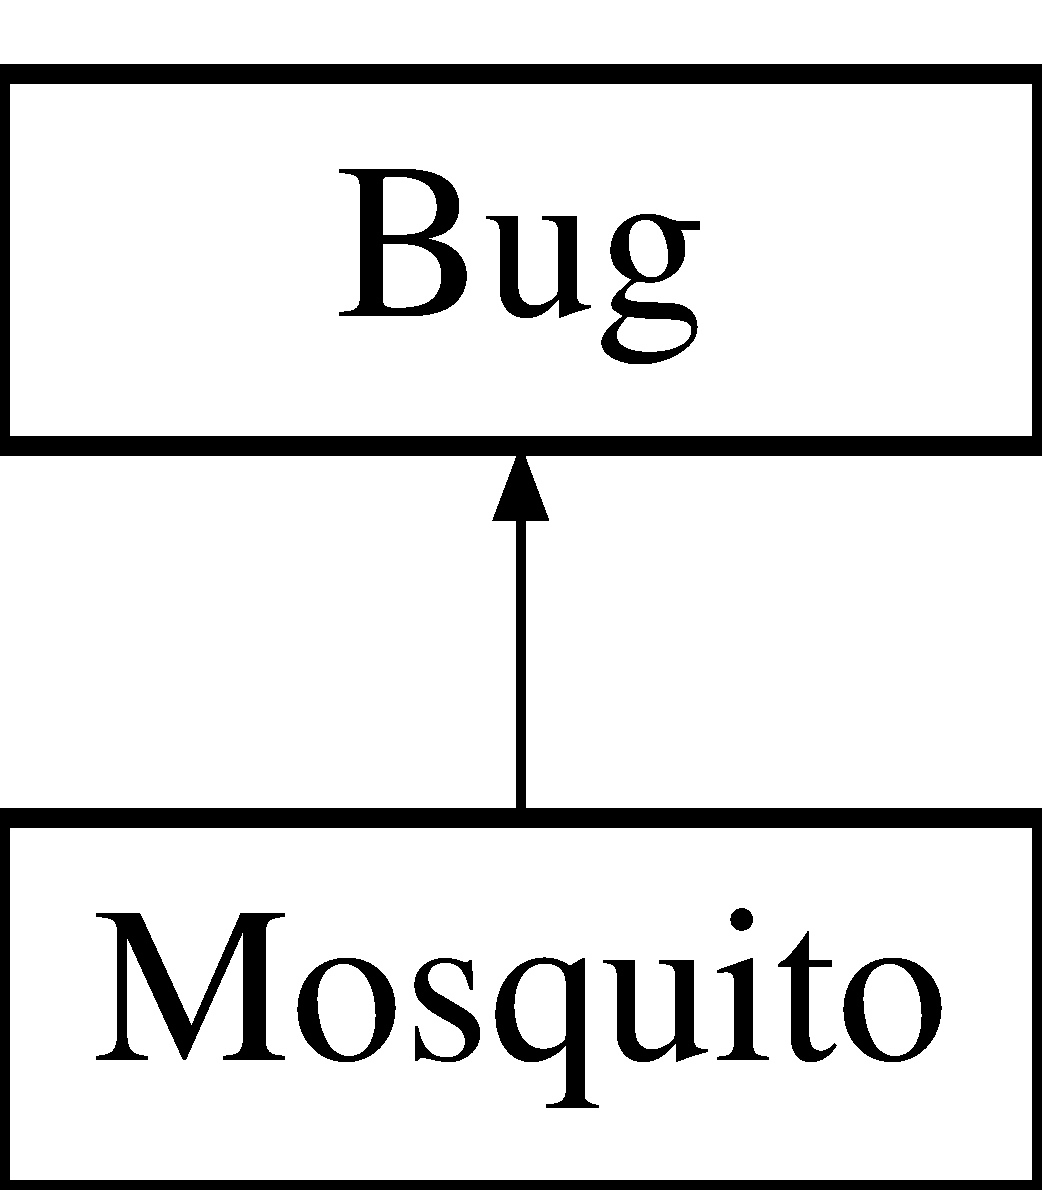
\includegraphics[height=2.000000cm]{classMosquito}
\end{center}
\end{figure}
\subsection*{Signaux}
\begin{DoxyCompactItemize}
\item 
void \hyperlink{classBug_ab7379f5a0172e2d536e20f3f29915e02}{dead} (\hyperlink{classBug}{Bug} $\ast$bug)
\begin{DoxyCompactList}\small\item\em Signal de mort de l'insecte. \end{DoxyCompactList}\item 
void \hyperlink{classBug_a33f90dffa55e1dce80dc2416c75a53c8}{goalReached} (\hyperlink{classBug}{Bug} $\ast$bug)
\begin{DoxyCompactList}\small\item\em Signal d'arrivé. \end{DoxyCompactList}\end{DoxyCompactItemize}
\subsection*{Fonctions membres publiques}
\begin{DoxyCompactItemize}
\item 
\hyperlink{classMosquito_ad7755ed5b7cd5ed184c5cfb2d4f0785d}{Mosquito} (double x, double y, double s, double start\_\-angle)
\begin{DoxyCompactList}\small\item\em Constructeur de \hyperlink{classMosquito}{Mosquito}. \end{DoxyCompactList}\item 
\hyperlink{classMosquito_aec4169f2175c544c8d6e119164b469cd}{$\sim$Mosquito} ()
\begin{DoxyCompactList}\small\item\em Destructeur de \hyperlink{classMosquito}{Mosquito}. \end{DoxyCompactList}\item 
void \hyperlink{classMosquito_a306ab9aefce1f42ae5d46746a018c845}{paint} (QPainter $\ast$painter, const QStyleOptionGraphicsItem $\ast$option, QWidget $\ast$widget)
\begin{DoxyCompactList}\small\item\em Surcharge de la fonction virtuelle pure \hyperlink{classMosquito_a306ab9aefce1f42ae5d46746a018c845}{paint()} hérité de QGraphicsObject. \end{DoxyCompactList}\item 
QRectF \hyperlink{classBug_a9b39c25361faad07b1bf2dd927d09dab}{boundingRect} () const 
\begin{DoxyCompactList}\small\item\em Surcharge de la fonction boudingRect() hérité de QGraphicsObject. \end{DoxyCompactList}\item 
QPainterPath \hyperlink{classBug_a587a36d3145c2b4dba6c689af22c65ac}{shape} () const 
\begin{DoxyCompactList}\small\item\em Surcharge de la fonction \hyperlink{classBug_a587a36d3145c2b4dba6c689af22c65ac}{shape()} hérité de QGraphicsObject. \end{DoxyCompactList}\item 
void \hyperlink{classBug_a63402c05b5ba3fb034e41f1ced0e4b9f}{hit} (double dmg)
\begin{DoxyCompactList}\small\item\em Infliger des dégats à l'insecte. \end{DoxyCompactList}\item 
short int \hyperlink{classBug_aced471cedcfa855baddf4c827003e755}{getMoveType} ()
\begin{DoxyCompactList}\small\item\em Permet d'accéder à la valeur moveType de l'insecte. \end{DoxyCompactList}\end{DoxyCompactItemize}
\subsection*{Champs de données}
\begin{DoxyCompactItemize}
\item 
\hyperlink{classRender}{Render} $\ast$ \hyperlink{classBug_a7a93aae4e4b7a215c94ff85d0bd6e26d}{parent}
\begin{DoxyCompactList}\small\item\em L'objet \hyperlink{classRender}{Render} parent de l'insecte. \end{DoxyCompactList}\end{DoxyCompactItemize}
\subsection*{Fonctions membres protégées}
\begin{DoxyCompactItemize}
\item 
void \hyperlink{classBug_a8e0ea03e85c9324a13328da60e5c52ee}{advance} (int step)
\begin{DoxyCompactList}\small\item\em Implémentation de la fonction virtuelle pure \hyperlink{classBug_a8e0ea03e85c9324a13328da60e5c52ee}{advance()} héritée de QGGaphicsObject. \end{DoxyCompactList}\end{DoxyCompactItemize}
\subsection*{Attributs protégés}
\begin{DoxyCompactItemize}
\item 
double \hyperlink{classBug_a27a0f0b84d15525e409955509e6e3c42}{size}
\begin{DoxyCompactList}\small\item\em Taille. \end{DoxyCompactList}\item 
int \hyperlink{classBug_ad7e3597cf049f1051be94fcaf2fd3598}{frame}
\begin{DoxyCompactList}\small\item\em Compteur de frame. \end{DoxyCompactList}\item 
double \hyperlink{classBug_a13b95fbf23748ea853b01bfd0b0e7fc8}{speed}
\begin{DoxyCompactList}\small\item\em Vitesse de base. \end{DoxyCompactList}\end{DoxyCompactItemize}
\subsection*{Attributs privés}
\begin{DoxyCompactItemize}
\item 
QImage $\ast$ \hyperlink{classMosquito_a8c451b0473a7d48ee0ed7de9627f46cb}{image} \mbox{[}2\mbox{]}
\begin{DoxyCompactList}\small\item\em Cache d'image. \end{DoxyCompactList}\end{DoxyCompactItemize}


\subsection{Description détaillée}
Définie les caractéristiques spécifiques aux moustiques, comme leur graphisme, leur type de déplacement (FLY)... 

\subsection{Documentation des constructeurs et destructeur}
\hypertarget{classMosquito_ad7755ed5b7cd5ed184c5cfb2d4f0785d}{
\index{Mosquito@{Mosquito}!Mosquito@{Mosquito}}
\index{Mosquito@{Mosquito}!Mosquito@{Mosquito}}
\subsubsection[{Mosquito}]{\setlength{\rightskip}{0pt plus 5cm}Mosquito::Mosquito (
\begin{DoxyParamCaption}
\item[{double}]{x, }
\item[{double}]{y, }
\item[{double}]{s, }
\item[{double}]{start\_\-angle}
\end{DoxyParamCaption}
)}}
\label{classMosquito_ad7755ed5b7cd5ed184c5cfb2d4f0785d}
Ce constructeur charge les images du moustique et appelle le constructeur parent de \hyperlink{classBug_a1d3140d50abd44257d5e0b1b6dcb4514}{Bug()} avec les paramètres correspondants aux caractéristiques d'un moustique. 
\begin{DoxyParams}{Paramètres}
{\em x} & Un double correspondant à l'abscisse du point de départ des insectes. \\
\hline
{\em y} & Un double correspondant à l'ordonnée du point de départ des insectes. \\
\hline
{\em s} & La taille du moustique, influe sur la taille de sa représentation graphique et sur les autres caractéristiques. \\
\hline
{\em start\_\-angle} & Angle de départ de l'insecte. \\
\hline
\end{DoxyParams}
\hypertarget{classMosquito_aec4169f2175c544c8d6e119164b469cd}{
\index{Mosquito@{Mosquito}!$\sim$Mosquito@{$\sim$Mosquito}}
\index{$\sim$Mosquito@{$\sim$Mosquito}!Mosquito@{Mosquito}}
\subsubsection[{$\sim$Mosquito}]{\setlength{\rightskip}{0pt plus 5cm}Mosquito::$\sim$Mosquito (
\begin{DoxyParamCaption}
{}
\end{DoxyParamCaption}
)}}
\label{classMosquito_aec4169f2175c544c8d6e119164b469cd}
Désalloue la mémoire des images du moustique mises en cache. 

\subsection{Documentation des fonctions membres}
\hypertarget{classBug_a8e0ea03e85c9324a13328da60e5c52ee}{
\index{Mosquito@{Mosquito}!advance@{advance}}
\index{advance@{advance}!Mosquito@{Mosquito}}
\subsubsection[{advance}]{\setlength{\rightskip}{0pt plus 5cm}void Bug::advance (
\begin{DoxyParamCaption}
\item[{int}]{step}
\end{DoxyParamCaption}
)\hspace{0.3cm}{\ttfamily  \mbox{[}protected, inherited\mbox{]}}}}
\label{classBug_a8e0ea03e85c9324a13328da60e5c52ee}
Implémentation de la fonction virtuelle pure \hyperlink{classBug_a8e0ea03e85c9324a13328da60e5c52ee}{advance()} héritée de QGGaphicsObject. 
\begin{DoxyParams}{Paramètres}
{\em step} & La fonction est appelé deux fois automatiquement par QT à chaque update(), une fois avec 0 comme paramètre puis une fois avec 1. \\
\hline
\end{DoxyParams}
\hypertarget{classBug_a9b39c25361faad07b1bf2dd927d09dab}{
\index{Mosquito@{Mosquito}!boundingRect@{boundingRect}}
\index{boundingRect@{boundingRect}!Mosquito@{Mosquito}}
\subsubsection[{boundingRect}]{\setlength{\rightskip}{0pt plus 5cm}QRectF Bug::boundingRect (
\begin{DoxyParamCaption}
{}
\end{DoxyParamCaption}
) const\hspace{0.3cm}{\ttfamily  \mbox{[}inherited\mbox{]}}}}
\label{classBug_a9b39c25361faad07b1bf2dd927d09dab}
Fonction appelé automatiquement par QT pour savoir s'il doit ou non réafficher l'insecte. \begin{DoxyReturn}{Renvoie}
Un objet QRectF correspondant au rectangle englobant l'ensemble du dessin de l'insecte. 
\end{DoxyReturn}
\hypertarget{classBug_ab7379f5a0172e2d536e20f3f29915e02}{
\index{Mosquito@{Mosquito}!dead@{dead}}
\index{dead@{dead}!Mosquito@{Mosquito}}
\subsubsection[{dead}]{\setlength{\rightskip}{0pt plus 5cm}void Bug::dead (
\begin{DoxyParamCaption}
\item[{{\bf Bug} $\ast$}]{bug}
\end{DoxyParamCaption}
)\hspace{0.3cm}{\ttfamily  \mbox{[}signal, inherited\mbox{]}}}}
\label{classBug_ab7379f5a0172e2d536e20f3f29915e02}
Signal émit lorsque l'insecte est tué. 
\begin{DoxyParams}{Paramètres}
{\em bug} & Un pointeur vers l'insecte qui vient de mourir. \\
\hline
\end{DoxyParams}
\hypertarget{classBug_aced471cedcfa855baddf4c827003e755}{
\index{Mosquito@{Mosquito}!getMoveType@{getMoveType}}
\index{getMoveType@{getMoveType}!Mosquito@{Mosquito}}
\subsubsection[{getMoveType}]{\setlength{\rightskip}{0pt plus 5cm}short int Bug::getMoveType (
\begin{DoxyParamCaption}
{}
\end{DoxyParamCaption}
)\hspace{0.3cm}{\ttfamily  \mbox{[}inherited\mbox{]}}}}
\label{classBug_aced471cedcfa855baddf4c827003e755}
\begin{DoxyReturn}{Renvoie}
la valeur prédéfinie FLY ou CRAWL. 
\end{DoxyReturn}
\hypertarget{classBug_a33f90dffa55e1dce80dc2416c75a53c8}{
\index{Mosquito@{Mosquito}!goalReached@{goalReached}}
\index{goalReached@{goalReached}!Mosquito@{Mosquito}}
\subsubsection[{goalReached}]{\setlength{\rightskip}{0pt plus 5cm}void Bug::goalReached (
\begin{DoxyParamCaption}
\item[{{\bf Bug} $\ast$}]{bug}
\end{DoxyParamCaption}
)\hspace{0.3cm}{\ttfamily  \mbox{[}signal, inherited\mbox{]}}}}
\label{classBug_a33f90dffa55e1dce80dc2416c75a53c8}
Signal émit par l'insecte lorsqu'il atteint son but. 
\begin{DoxyParams}{Paramètres}
{\em bug} & Un pointeur vers l'insecte. \\
\hline
\end{DoxyParams}
\hypertarget{classBug_a63402c05b5ba3fb034e41f1ced0e4b9f}{
\index{Mosquito@{Mosquito}!hit@{hit}}
\index{hit@{hit}!Mosquito@{Mosquito}}
\subsubsection[{hit}]{\setlength{\rightskip}{0pt plus 5cm}void Bug::hit (
\begin{DoxyParamCaption}
\item[{double}]{dmg}
\end{DoxyParamCaption}
)\hspace{0.3cm}{\ttfamily  \mbox{[}inherited\mbox{]}}}}
\label{classBug_a63402c05b5ba3fb034e41f1ced0e4b9f}
Fonction pouvant être appelée pour infliger des dégats à l'insecte (par exemple par les projectiles des tours). 
\begin{DoxyParams}{Paramètres}
{\em dmg} & Un double correspondant au point de dégat à infliger (avant réduction par la résistance de l'insecte). \\
\hline
\end{DoxyParams}


Réimplémentée dans \hyperlink{classAnt_a64b0e0e7d2605c1a5a0906587ab70920}{Ant}.

\hypertarget{classMosquito_a306ab9aefce1f42ae5d46746a018c845}{
\index{Mosquito@{Mosquito}!paint@{paint}}
\index{paint@{paint}!Mosquito@{Mosquito}}
\subsubsection[{paint}]{\setlength{\rightskip}{0pt plus 5cm}void Mosquito::paint (
\begin{DoxyParamCaption}
\item[{QPainter $\ast$}]{painter, }
\item[{const QStyleOptionGraphicsItem $\ast$}]{option, }
\item[{QWidget $\ast$}]{widget}
\end{DoxyParamCaption}
)}}
\label{classMosquito_a306ab9aefce1f42ae5d46746a018c845}
Est appelé automatiquement par Qt pour redessiner le moustique. \hypertarget{classBug_a587a36d3145c2b4dba6c689af22c65ac}{
\index{Mosquito@{Mosquito}!shape@{shape}}
\index{shape@{shape}!Mosquito@{Mosquito}}
\subsubsection[{shape}]{\setlength{\rightskip}{0pt plus 5cm}QPainterPath Bug::shape (
\begin{DoxyParamCaption}
{}
\end{DoxyParamCaption}
) const\hspace{0.3cm}{\ttfamily  \mbox{[}inherited\mbox{]}}}}
\label{classBug_a587a36d3145c2b4dba6c689af22c65ac}
Fonction utilisé par QT pour traiter les collisions entre objets graphiques. \begin{DoxyReturn}{Renvoie}
Un object QPainterPath correspondant au contour de collision de l'insecte. 
\end{DoxyReturn}


\subsection{Documentation des champs}
\hypertarget{classBug_ad7e3597cf049f1051be94fcaf2fd3598}{
\index{Mosquito@{Mosquito}!frame@{frame}}
\index{frame@{frame}!Mosquito@{Mosquito}}
\subsubsection[{frame}]{\setlength{\rightskip}{0pt plus 5cm}int {\bf Bug::frame}\hspace{0.3cm}{\ttfamily  \mbox{[}protected, inherited\mbox{]}}}}
\label{classBug_ad7e3597cf049f1051be94fcaf2fd3598}
Compteur d'image utilisé pour afficher successivement chaque image des animations. \hypertarget{classMosquito_a8c451b0473a7d48ee0ed7de9627f46cb}{
\index{Mosquito@{Mosquito}!image@{image}}
\index{image@{image}!Mosquito@{Mosquito}}
\subsubsection[{image}]{\setlength{\rightskip}{0pt plus 5cm}QImage$\ast$ {\bf Mosquito::image}\mbox{[}2\mbox{]}\hspace{0.3cm}{\ttfamily  \mbox{[}private\mbox{]}}}}
\label{classMosquito_a8c451b0473a7d48ee0ed7de9627f46cb}
Les images du moustique sont redimensionnées puis mises en cache pour un affichage plus rapide. \hypertarget{classBug_a7a93aae4e4b7a215c94ff85d0bd6e26d}{
\index{Mosquito@{Mosquito}!parent@{parent}}
\index{parent@{parent}!Mosquito@{Mosquito}}
\subsubsection[{parent}]{\setlength{\rightskip}{0pt plus 5cm}{\bf Render}$\ast$ {\bf Bug::parent}\hspace{0.3cm}{\ttfamily  \mbox{[}inherited\mbox{]}}}}
\label{classBug_a7a93aae4e4b7a215c94ff85d0bd6e26d}
Quand on ajoute un insecte à l'objet \hyperlink{classRender}{Render} par la méthode addBug(), cet attribut est automatiquement initialisé. \hypertarget{classBug_a27a0f0b84d15525e409955509e6e3c42}{
\index{Mosquito@{Mosquito}!size@{size}}
\index{size@{size}!Mosquito@{Mosquito}}
\subsubsection[{size}]{\setlength{\rightskip}{0pt plus 5cm}double {\bf Bug::size}\hspace{0.3cm}{\ttfamily  \mbox{[}protected, inherited\mbox{]}}}}
\label{classBug_a27a0f0b84d15525e409955509e6e3c42}
La taille de l'insecte, influe à la fois sur la taille de la représentation graphique et sur les caractéristiques de l'insecte.' \hypertarget{classBug_a13b95fbf23748ea853b01bfd0b0e7fc8}{
\index{Mosquito@{Mosquito}!speed@{speed}}
\index{speed@{speed}!Mosquito@{Mosquito}}
\subsubsection[{speed}]{\setlength{\rightskip}{0pt plus 5cm}double {\bf Bug::speed}\hspace{0.3cm}{\ttfamily  \mbox{[}protected, inherited\mbox{]}}}}
\label{classBug_a13b95fbf23748ea853b01bfd0b0e7fc8}
La vitesse en case/seconde à laquelle se déplace l'insecte. 

La documentation de cette classe a été générée à partir des fichiers suivants :\begin{DoxyCompactItemize}
\item 
src/Mosquito.h\item 
src/Mosquito.cpp\end{DoxyCompactItemize}

\hypertarget{classProjectile}{
\section{Référence de la classe Projectile}
\label{classProjectile}\index{Projectile@{Projectile}}
}


Classe représentant les projectiles des tours.  




{\ttfamily \#include $<$Projectile.h$>$}

Graphe d'héritage de Projectile:\begin{figure}[H]
\begin{center}
\leavevmode
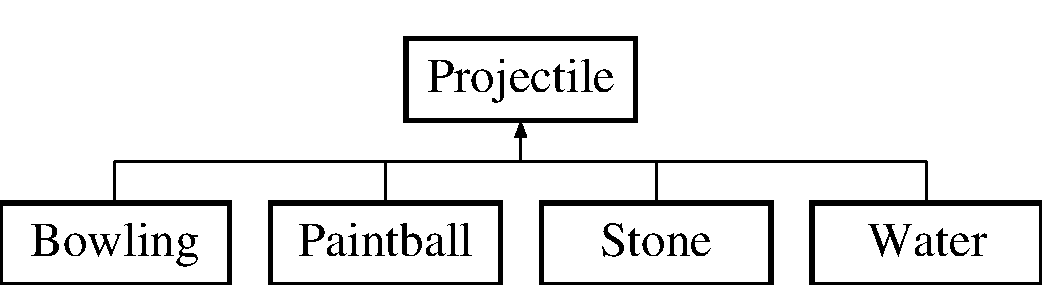
\includegraphics[height=2.000000cm]{classProjectile}
\end{center}
\end{figure}
\subsection*{Signaux}
\begin{DoxyCompactItemize}
\item 
void \hyperlink{classProjectile_a18d1fccd74f92b54f239c13c74cbc00c}{explode} (\hyperlink{classProjectile}{Projectile} $\ast$missile)
\begin{DoxyCompactList}\small\item\em Signal d'explosion du projectile. \end{DoxyCompactList}\end{DoxyCompactItemize}
\subsection*{Fonctions membres publiques}
\begin{DoxyCompactItemize}
\item 
\hyperlink{classProjectile_adb1e35e75922feb87c3391f549d3274f}{Projectile} (QPointF start, \hyperlink{classBug}{Bug} $\ast$trgt, double init\_\-speed, double damage)
\begin{DoxyCompactList}\small\item\em Constructeur de \hyperlink{classProjectile}{Projectile} Initialise les caractéristiques du projectile. \end{DoxyCompactList}\item 
QRectF \hyperlink{classProjectile_a0e0b18909c9c154404384707c6515802}{boundingRect} () const 
\begin{DoxyCompactList}\small\item\em Surcharge de la methode virtuelle pure \hyperlink{classProjectile_a0e0b18909c9c154404384707c6515802}{boundingRect()} héritée de QGraphicsObject. \end{DoxyCompactList}\item 
void \hyperlink{classProjectile_aef0d6ffcea7620988cf5446d0c1133fa}{paint} (QPainter $\ast$painter, QColor color)
\begin{DoxyCompactList}\small\item\em Surcharge de la méthode virtuelle pure \hyperlink{classProjectile_aef0d6ffcea7620988cf5446d0c1133fa}{paint()} héritée de QGraphicsObject. \end{DoxyCompactList}\end{DoxyCompactItemize}
\subsection*{Fonctions membres protégées}
\begin{DoxyCompactItemize}
\item 
void \hyperlink{classProjectile_a8e3b4bae49558a0febfce8c1accea72d}{advance} (int step)
\begin{DoxyCompactList}\small\item\em Surcharge de la méthode virtuelle pure héritée de QGraphicsObject. \end{DoxyCompactList}\end{DoxyCompactItemize}
\subsection*{Attributs privés}
\begin{DoxyCompactItemize}
\item 
QPointF \hyperlink{classProjectile_a15091a3a02fbfac2dd4fb44ac9cbceab}{dest}
\begin{DoxyCompactList}\small\item\em La destination du projectile. \end{DoxyCompactList}\item 
\hyperlink{classBug}{Bug} $\ast$ \hyperlink{classProjectile_ae5273bd2c6550b94f38310b69859b093}{target}
\begin{DoxyCompactList}\small\item\em L'insecte ciblée par le projectile. \end{DoxyCompactList}\item 
double \hyperlink{classProjectile_aae1f5d683c71d152b6a12d922ec4714f}{speed}
\begin{DoxyCompactList}\small\item\em La vitesse en case par seconde du projectile. \end{DoxyCompactList}\item 
double \hyperlink{classProjectile_ac94938ed5b3d3e01217bf72f80ad2e3d}{dmg}
\begin{DoxyCompactList}\small\item\em Les dégats infligé à l'impact par le projectile. \end{DoxyCompactList}\item 
double \hyperlink{classProjectile_a019db4c89ccf3eb291b06ba7b55f0754}{maxrange}
\begin{DoxyCompactList}\small\item\em La portée maximale du projectile (s'il n'atteint personne avant d'arriver à se portée max, il disparait). \end{DoxyCompactList}\item 
double \hyperlink{classProjectile_a0fc0c0258f36a9347f45d1edb8b767e5}{travelled}
\begin{DoxyCompactList}\small\item\em La distance parcourue par le projectile. \end{DoxyCompactList}\end{DoxyCompactItemize}


\subsection{Description détaillée}
Définie les méthodes des projectiles ainsi que leur caractéristiques de base. 

\subsection{Documentation des constructeurs et destructeur}
\hypertarget{classProjectile_adb1e35e75922feb87c3391f549d3274f}{
\index{Projectile@{Projectile}!Projectile@{Projectile}}
\index{Projectile@{Projectile}!Projectile@{Projectile}}
\subsubsection[{Projectile}]{\setlength{\rightskip}{0pt plus 5cm}Projectile::Projectile (
\begin{DoxyParamCaption}
\item[{QPointF}]{start, }
\item[{{\bf Bug} $\ast$}]{trgt, }
\item[{double}]{init\_\-speed, }
\item[{double}]{damage}
\end{DoxyParamCaption}
)}}
\label{classProjectile_adb1e35e75922feb87c3391f549d3274f}

\begin{DoxyParams}{Paramètres}
{\em start} & Point de départ du projectile. \\
\hline
{\em trgt} & Insecte cible du projectile. \\
\hline
{\em init\_\-speed} & Vitesse de vol du projectile. \\
\hline
{\em damage} & Dégats infligés à l'impact par le projectile. \\
\hline
\end{DoxyParams}


\subsection{Documentation des fonctions membres}
\hypertarget{classProjectile_a8e3b4bae49558a0febfce8c1accea72d}{
\index{Projectile@{Projectile}!advance@{advance}}
\index{advance@{advance}!Projectile@{Projectile}}
\subsubsection[{advance}]{\setlength{\rightskip}{0pt plus 5cm}void Projectile::advance (
\begin{DoxyParamCaption}
\item[{int}]{step}
\end{DoxyParamCaption}
)\hspace{0.3cm}{\ttfamily  \mbox{[}protected\mbox{]}}}}
\label{classProjectile_a8e3b4bae49558a0febfce8c1accea72d}
Est appellé automatiquement par Qt deux fois par appelle au slot advance de la QGraphicsScene. 
\begin{DoxyParams}{Paramètres}
{\em step} & appelé une fois avant de redessiner avec step = 0 et une fois avec step = 1. \\
\hline
\end{DoxyParams}
\hypertarget{classProjectile_a0e0b18909c9c154404384707c6515802}{
\index{Projectile@{Projectile}!boundingRect@{boundingRect}}
\index{boundingRect@{boundingRect}!Projectile@{Projectile}}
\subsubsection[{boundingRect}]{\setlength{\rightskip}{0pt plus 5cm}QRectF Projectile::boundingRect (
\begin{DoxyParamCaption}
{}
\end{DoxyParamCaption}
) const}}
\label{classProjectile_a0e0b18909c9c154404384707c6515802}
Fonction appelé automatiquement par QT pour savoir s'il doit redessiner ou non l'objet graphique. \begin{DoxyReturn}{Renvoie}
Un object QRectF correspondant au rectangle englobant le dessin du projectile. 
\end{DoxyReturn}
\hypertarget{classProjectile_a18d1fccd74f92b54f239c13c74cbc00c}{
\index{Projectile@{Projectile}!explode@{explode}}
\index{explode@{explode}!Projectile@{Projectile}}
\subsubsection[{explode}]{\setlength{\rightskip}{0pt plus 5cm}void Projectile::explode (
\begin{DoxyParamCaption}
\item[{{\bf Projectile} $\ast$}]{missile}
\end{DoxyParamCaption}
)\hspace{0.3cm}{\ttfamily  \mbox{[}signal\mbox{]}}}}
\label{classProjectile_a18d1fccd74f92b54f239c13c74cbc00c}
Signale émit lorsque le projectile explose pour qu'il soit retiré de la scène. 
\begin{DoxyParams}{Paramètres}
{\em missile} & Un pointeur vers le projectile pour que la scène puisse le détruire correctement. \\
\hline
\end{DoxyParams}
\hypertarget{classProjectile_aef0d6ffcea7620988cf5446d0c1133fa}{
\index{Projectile@{Projectile}!paint@{paint}}
\index{paint@{paint}!Projectile@{Projectile}}
\subsubsection[{paint}]{\setlength{\rightskip}{0pt plus 5cm}void Projectile::paint (
\begin{DoxyParamCaption}
\item[{QPainter $\ast$}]{painter, }
\item[{QColor}]{color}
\end{DoxyParamCaption}
)}}
\label{classProjectile_aef0d6ffcea7620988cf5446d0c1133fa}
Est appelé automatiquement par Qt pour redessiner le projectile. 

\subsection{Documentation des champs}
\hypertarget{classProjectile_a15091a3a02fbfac2dd4fb44ac9cbceab}{
\index{Projectile@{Projectile}!dest@{dest}}
\index{dest@{dest}!Projectile@{Projectile}}
\subsubsection[{dest}]{\setlength{\rightskip}{0pt plus 5cm}QPointF {\bf Projectile::dest}\hspace{0.3cm}{\ttfamily  \mbox{[}private\mbox{]}}}}
\label{classProjectile_a15091a3a02fbfac2dd4fb44ac9cbceab}
\hypertarget{classProjectile_ac94938ed5b3d3e01217bf72f80ad2e3d}{
\index{Projectile@{Projectile}!dmg@{dmg}}
\index{dmg@{dmg}!Projectile@{Projectile}}
\subsubsection[{dmg}]{\setlength{\rightskip}{0pt plus 5cm}double {\bf Projectile::dmg}\hspace{0.3cm}{\ttfamily  \mbox{[}private\mbox{]}}}}
\label{classProjectile_ac94938ed5b3d3e01217bf72f80ad2e3d}
\hypertarget{classProjectile_a019db4c89ccf3eb291b06ba7b55f0754}{
\index{Projectile@{Projectile}!maxrange@{maxrange}}
\index{maxrange@{maxrange}!Projectile@{Projectile}}
\subsubsection[{maxrange}]{\setlength{\rightskip}{0pt plus 5cm}double {\bf Projectile::maxrange}\hspace{0.3cm}{\ttfamily  \mbox{[}private\mbox{]}}}}
\label{classProjectile_a019db4c89ccf3eb291b06ba7b55f0754}
\hypertarget{classProjectile_aae1f5d683c71d152b6a12d922ec4714f}{
\index{Projectile@{Projectile}!speed@{speed}}
\index{speed@{speed}!Projectile@{Projectile}}
\subsubsection[{speed}]{\setlength{\rightskip}{0pt plus 5cm}double {\bf Projectile::speed}\hspace{0.3cm}{\ttfamily  \mbox{[}private\mbox{]}}}}
\label{classProjectile_aae1f5d683c71d152b6a12d922ec4714f}
\hypertarget{classProjectile_ae5273bd2c6550b94f38310b69859b093}{
\index{Projectile@{Projectile}!target@{target}}
\index{target@{target}!Projectile@{Projectile}}
\subsubsection[{target}]{\setlength{\rightskip}{0pt plus 5cm}{\bf Bug}$\ast$ {\bf Projectile::target}\hspace{0.3cm}{\ttfamily  \mbox{[}private\mbox{]}}}}
\label{classProjectile_ae5273bd2c6550b94f38310b69859b093}
\hypertarget{classProjectile_a0fc0c0258f36a9347f45d1edb8b767e5}{
\index{Projectile@{Projectile}!travelled@{travelled}}
\index{travelled@{travelled}!Projectile@{Projectile}}
\subsubsection[{travelled}]{\setlength{\rightskip}{0pt plus 5cm}double {\bf Projectile::travelled}\hspace{0.3cm}{\ttfamily  \mbox{[}private\mbox{]}}}}
\label{classProjectile_a0fc0c0258f36a9347f45d1edb8b767e5}


La documentation de cette classe a été générée à partir des fichiers suivants :\begin{DoxyCompactItemize}
\item 
src/Projectile.h\item 
src/moc\_\-Projectile.cpp\item 
src/Projectile.cpp\end{DoxyCompactItemize}

\hypertarget{classRender}{
\section{Référence de la classe Render}
\label{classRender}\index{Render@{Render}}
}
\subsection*{Connecteurs publics}
\begin{DoxyCompactItemize}
\item 
\hypertarget{classRender_a3252d02e9509f342bc96129b4b10b415}{
void {\bfseries nextWave} ()}
\label{classRender_a3252d02e9509f342bc96129b4b10b415}

\item 
\hypertarget{classRender_a9413625fc472b4b7806f3a0d615d6ea9}{
void {\bfseries nextBug} ()}
\label{classRender_a9413625fc472b4b7806f3a0d615d6ea9}

\item 
\hypertarget{classRender_a8e2eccb2fc3914198b8939bf0625c955}{
void {\bfseries towerBought} (QString type)}
\label{classRender_a8e2eccb2fc3914198b8939bf0625c955}

\item 
\hypertarget{classRender_aeeddbbe27102625cc2d5234fa0be523a}{
void {\bfseries bugFinish} (\hyperlink{classBug}{Bug} $\ast$bug)}
\label{classRender_aeeddbbe27102625cc2d5234fa0be523a}

\item 
\hypertarget{classRender_a940007358a139d0b30e002929d24f770}{
void {\bfseries bugKilled} (\hyperlink{classBug}{Bug} $\ast$bug)}
\label{classRender_a940007358a139d0b30e002929d24f770}

\item 
\hypertarget{classRender_a3b5bb3705131ca57252398e0f6a9e3e5}{
void {\bfseries addProjectile} (\hyperlink{classProjectile}{Projectile} $\ast$missile)}
\label{classRender_a3b5bb3705131ca57252398e0f6a9e3e5}

\item 
\hypertarget{classRender_a20678c257926bfff635fded745e11f4a}{
void {\bfseries destroyTower} (\hyperlink{classTower}{Tower} $\ast$tower)}
\label{classRender_a20678c257926bfff635fded745e11f4a}

\end{DoxyCompactItemize}
\subsection*{Signaux}
\begin{DoxyCompactItemize}
\item 
\hypertarget{classRender_a916c15ab4b31cc0f34d9d53b89b89ac0}{
void {\bfseries newWaveName} (QString name)}
\label{classRender_a916c15ab4b31cc0f34d9d53b89b89ac0}

\item 
\hypertarget{classRender_ad88f7f01a7b9fafa756221707d590a78}{
void {\bfseries loseLife} ()}
\label{classRender_ad88f7f01a7b9fafa756221707d590a78}

\item 
\hypertarget{classRender_acd71f1c6c9d67dff3627da4ff6a4c9b8}{
void {\bfseries getCred} ()}
\label{classRender_acd71f1c6c9d67dff3627da4ff6a4c9b8}

\item 
\hypertarget{classRender_a126c4b49e93103a751f66359d8e63171}{
void {\bfseries selectTower} (\hyperlink{classTower}{Tower} $\ast$tower)}
\label{classRender_a126c4b49e93103a751f66359d8e63171}

\end{DoxyCompactItemize}
\subsection*{Fonctions membres publiques}
\begin{DoxyCompactItemize}
\item 
\hypertarget{classRender_aae10ca06c2755038752a2a007727f0ca}{
void {\bfseries drawBackground} (QPainter $\ast$painter, const QRectF \&rect)}
\label{classRender_aae10ca06c2755038752a2a007727f0ca}

\item 
\hypertarget{classRender_a1291eebbb0647502fc90d058bc22e7a3}{
QPoint {\bfseries square} (QGraphicsItem \&item)}
\label{classRender_a1291eebbb0647502fc90d058bc22e7a3}

\item 
\hypertarget{classRender_afd1f727c1514ca01ad1cefbf4992497b}{
QPoint {\bfseries goal} ()}
\label{classRender_afd1f727c1514ca01ad1cefbf4992497b}

\item 
\hypertarget{classRender_a696f385b556f15a7420293a055734e4d}{
double {\bfseries getAngle} (QPoint \&current)}
\label{classRender_a696f385b556f15a7420293a055734e4d}

\item 
\hypertarget{classRender_a899ce19de8a01bb4bc01653cd8761357}{
void {\bfseries mousePressEvent} (QGraphicsSceneMouseEvent $\ast$mouseEvent)}
\label{classRender_a899ce19de8a01bb4bc01653cd8761357}

\item 
\hypertarget{classRender_a3cb540a53c73c9febbee2e4b11ea1077}{
\hyperlink{classBug}{Bug} $\ast$ {\bfseries getTarget} (QPointF pos, double range)}
\label{classRender_a3cb540a53c73c9febbee2e4b11ea1077}

\end{DoxyCompactItemize}
\subsection*{Fonctions membres privées}
\begin{DoxyCompactItemize}
\item 
\hypertarget{classRender_a4a1fed13f76997e45e90dd39d622d33e}{
void {\bfseries addBug} (\hyperlink{classBug}{Bug} $\ast$bug)}
\label{classRender_a4a1fed13f76997e45e90dd39d622d33e}

\end{DoxyCompactItemize}
\subsection*{Attributs privés}
\begin{DoxyCompactItemize}
\item 
\hypertarget{classRender_a6351bb3de99ef093995785788c1d218e}{
QTimer {\bfseries waveTimer}}
\label{classRender_a6351bb3de99ef093995785788c1d218e}

\item 
\hypertarget{classRender_afa2c3b6d106bf91639ddf351d7d3315e}{
QPoint $\ast$ {\bfseries start}}
\label{classRender_afa2c3b6d106bf91639ddf351d7d3315e}

\item 
\hypertarget{classRender_ab66f1b35519a6e9d6fe14e75a6973680}{
double {\bfseries start\_\-angle}}
\label{classRender_ab66f1b35519a6e9d6fe14e75a6973680}

\item 
\hypertarget{classRender_a682e96907f3d52f710df4e9c2a5e9d07}{
int {\bfseries waveNumber}}
\label{classRender_a682e96907f3d52f710df4e9c2a5e9d07}

\item 
\hypertarget{classRender_a6b5e2349a706152d4763d22b995e9237}{
QStringList $\ast$ {\bfseries wave}}
\label{classRender_a6b5e2349a706152d4763d22b995e9237}

\item 
\hypertarget{classRender_a9c7793879c5007b8cae3a9c2885d283f}{
int {\bfseries map} \mbox{[}ROW\mbox{]}\mbox{[}COLUMN\mbox{]}}
\label{classRender_a9c7793879c5007b8cae3a9c2885d283f}

\item 
\hypertarget{classRender_a7b01b65692570fe6dec24d0a5c1aa178}{
\hyperlink{classTower}{Tower} $\ast$ {\bfseries towers} \mbox{[}ROW\mbox{]}\mbox{[}COLUMN\mbox{]}}
\label{classRender_a7b01b65692570fe6dec24d0a5c1aa178}

\item 
\hypertarget{classRender_a08247005a2c595988f8a0ab14a8b1ad9}{
QPoint {\bfseries goalSquare}}
\label{classRender_a08247005a2c595988f8a0ab14a8b1ad9}

\item 
\hypertarget{classRender_aaa10cde2c7a766914312f85d7c7eb25c}{
QHash$<$ int, QPixmap $>$ {\bfseries tiles}}
\label{classRender_aaa10cde2c7a766914312f85d7c7eb25c}

\item 
\hypertarget{classRender_ac6b86ad92172fefa5b9a56b31e9055d3}{
\hyperlink{classHatchery}{Hatchery} $\ast$ {\bfseries b1}}
\label{classRender_ac6b86ad92172fefa5b9a56b31e9055d3}

\item 
\hypertarget{classRender_ae8f2c323913fe8b89e0e7f443ef41ae0}{
QString {\bfseries tower2build}}
\label{classRender_ae8f2c323913fe8b89e0e7f443ef41ae0}

\item 
\hypertarget{classRender_a3d5b29479d129b61c6ad8f3eec2f1f76}{
QList$<$ \hyperlink{classBug}{Bug} $\ast$ $>$ {\bfseries bugs}}
\label{classRender_a3d5b29479d129b61c6ad8f3eec2f1f76}

\end{DoxyCompactItemize}


La documentation de cette classe a été générée à partir des fichiers suivants :\begin{DoxyCompactItemize}
\item 
src/Render.h\item 
src/moc\_\-Render.cpp\item 
src/Render.cpp\end{DoxyCompactItemize}

\hypertarget{classRoach}{
\section{Référence de la classe Roach}
\label{classRoach}\index{Roach@{Roach}}
}
Graphe d'héritage de Roach:\begin{figure}[H]
\begin{center}
\leavevmode
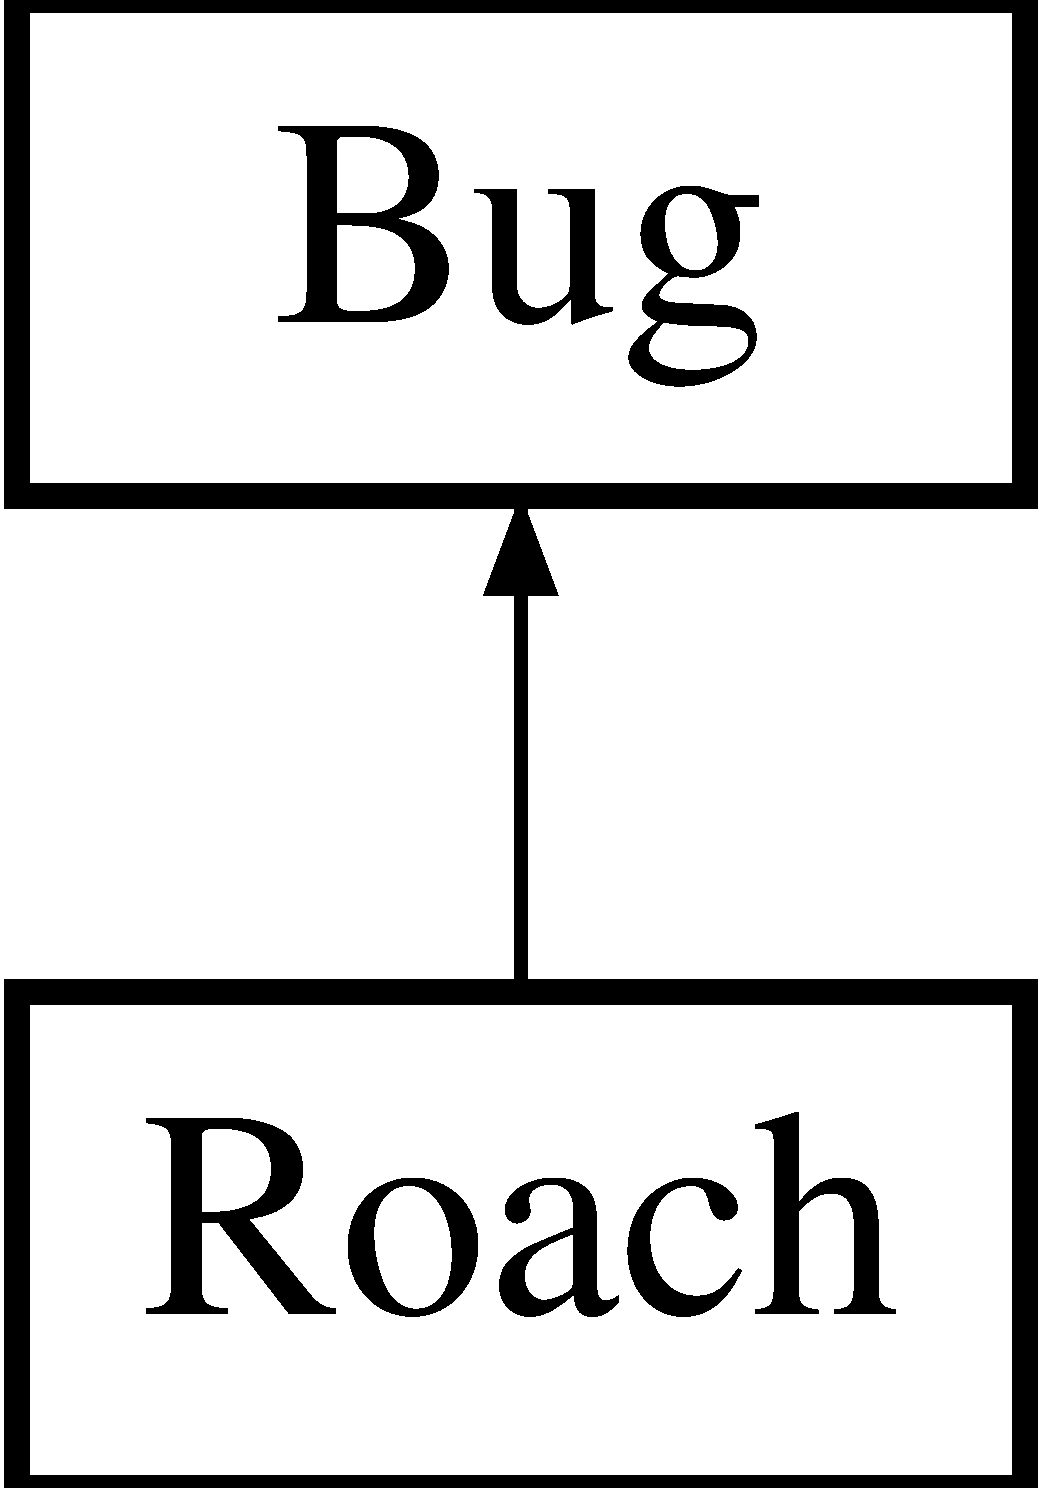
\includegraphics[height=2.000000cm]{classRoach}
\end{center}
\end{figure}
\subsection*{Signaux}
\begin{DoxyCompactItemize}
\item 
void \hyperlink{classBug_ab7379f5a0172e2d536e20f3f29915e02}{dead} (\hyperlink{classBug}{Bug} $\ast$bug)
\begin{DoxyCompactList}\small\item\em Signal de mort de l'insecte. \end{DoxyCompactList}\item 
void \hyperlink{classBug_a33f90dffa55e1dce80dc2416c75a53c8}{goalReached} (\hyperlink{classBug}{Bug} $\ast$bug)
\begin{DoxyCompactList}\small\item\em Signal d'arrivé. \end{DoxyCompactList}\end{DoxyCompactItemize}
\subsection*{Fonctions membres publiques}
\begin{DoxyCompactItemize}
\item 
\hypertarget{classRoach_af12999aec092cc5dc1afb0c3f85ee353}{
{\bfseries Roach} (double x, double y, double s, double start\_\-angle)}
\label{classRoach_af12999aec092cc5dc1afb0c3f85ee353}

\item 
\hypertarget{classRoach_a13a922274476d77e17405cbe199ce691}{
void {\bfseries paint} (QPainter $\ast$painter, const QStyleOptionGraphicsItem $\ast$option, QWidget $\ast$widget)}
\label{classRoach_a13a922274476d77e17405cbe199ce691}

\item 
QRectF \hyperlink{classBug_a9b39c25361faad07b1bf2dd927d09dab}{boundingRect} () const 
\begin{DoxyCompactList}\small\item\em Surcharge de la fonction boudingRect() hérité de QGraphicsObject. \end{DoxyCompactList}\item 
QPainterPath \hyperlink{classBug_a587a36d3145c2b4dba6c689af22c65ac}{shape} () const 
\begin{DoxyCompactList}\small\item\em Surcharge de la fonction \hyperlink{classBug_a587a36d3145c2b4dba6c689af22c65ac}{shape()} hérité de QGraphicsObject. \end{DoxyCompactList}\item 
void \hyperlink{classBug_a63402c05b5ba3fb034e41f1ced0e4b9f}{hit} (double dmg)
\begin{DoxyCompactList}\small\item\em Infliger des dégats à l'insecte. \end{DoxyCompactList}\item 
short int \hyperlink{classBug_aced471cedcfa855baddf4c827003e755}{getMoveType} ()
\begin{DoxyCompactList}\small\item\em Permet d'accéder à la valeur moveType de l'insecte. \end{DoxyCompactList}\end{DoxyCompactItemize}
\subsection*{Champs de données}
\begin{DoxyCompactItemize}
\item 
\hyperlink{classRender}{Render} $\ast$ \hyperlink{classBug_a7a93aae4e4b7a215c94ff85d0bd6e26d}{parent}
\begin{DoxyCompactList}\small\item\em L'objet \hyperlink{classRender}{Render} parent de l'insecte. \end{DoxyCompactList}\end{DoxyCompactItemize}
\subsection*{Fonctions membres protégées}
\begin{DoxyCompactItemize}
\item 
void \hyperlink{classBug_a8e0ea03e85c9324a13328da60e5c52ee}{advance} (int step)
\begin{DoxyCompactList}\small\item\em Implémentation de la fonction virtuelle pure \hyperlink{classBug_a8e0ea03e85c9324a13328da60e5c52ee}{advance()} héritée de QGGaphicsObject. \end{DoxyCompactList}\end{DoxyCompactItemize}
\subsection*{Attributs protégés}
\begin{DoxyCompactItemize}
\item 
double \hyperlink{classBug_a27a0f0b84d15525e409955509e6e3c42}{size}
\begin{DoxyCompactList}\small\item\em Taille. \end{DoxyCompactList}\item 
int \hyperlink{classBug_ad7e3597cf049f1051be94fcaf2fd3598}{frame}
\begin{DoxyCompactList}\small\item\em Compteur de frame. \end{DoxyCompactList}\item 
double \hyperlink{classBug_a13b95fbf23748ea853b01bfd0b0e7fc8}{speed}
\begin{DoxyCompactList}\small\item\em Vitesse de base. \end{DoxyCompactList}\end{DoxyCompactItemize}
\subsection*{Attributs privés}
\begin{DoxyCompactItemize}
\item 
\hypertarget{classRoach_afe6b72503197eb2bacafda9df317b96f}{
QImage $\ast$ {\bfseries image} \mbox{[}3\mbox{]}}
\label{classRoach_afe6b72503197eb2bacafda9df317b96f}

\end{DoxyCompactItemize}


\subsection{Documentation des fonctions membres}
\hypertarget{classBug_a8e0ea03e85c9324a13328da60e5c52ee}{
\index{Roach@{Roach}!advance@{advance}}
\index{advance@{advance}!Roach@{Roach}}
\subsubsection[{advance}]{\setlength{\rightskip}{0pt plus 5cm}void Bug::advance (
\begin{DoxyParamCaption}
\item[{int}]{step}
\end{DoxyParamCaption}
)\hspace{0.3cm}{\ttfamily  \mbox{[}protected, inherited\mbox{]}}}}
\label{classBug_a8e0ea03e85c9324a13328da60e5c52ee}
Implémentation de la fonction virtuelle pure \hyperlink{classBug_a8e0ea03e85c9324a13328da60e5c52ee}{advance()} héritée de QGGaphicsObject. 
\begin{DoxyParams}{Paramètres}
{\em step} & La fonction est appelé deux fois automatiquement par QT à chaque update(), une fois avec 0 comme paramètre puis une fois avec 1. \\
\hline
\end{DoxyParams}
\hypertarget{classBug_a9b39c25361faad07b1bf2dd927d09dab}{
\index{Roach@{Roach}!boundingRect@{boundingRect}}
\index{boundingRect@{boundingRect}!Roach@{Roach}}
\subsubsection[{boundingRect}]{\setlength{\rightskip}{0pt plus 5cm}QRectF Bug::boundingRect (
\begin{DoxyParamCaption}
{}
\end{DoxyParamCaption}
) const\hspace{0.3cm}{\ttfamily  \mbox{[}inherited\mbox{]}}}}
\label{classBug_a9b39c25361faad07b1bf2dd927d09dab}
Fonction appelé automatiquement par QT pour savoir s'il doit ou non réafficher l'insecte. \begin{DoxyReturn}{Renvoie}
Un objet QRectF correspondant au rectangle englobant l'ensemble du dessin de l'insecte. 
\end{DoxyReturn}
\hypertarget{classBug_ab7379f5a0172e2d536e20f3f29915e02}{
\index{Roach@{Roach}!dead@{dead}}
\index{dead@{dead}!Roach@{Roach}}
\subsubsection[{dead}]{\setlength{\rightskip}{0pt plus 5cm}void Bug::dead (
\begin{DoxyParamCaption}
\item[{{\bf Bug} $\ast$}]{bug}
\end{DoxyParamCaption}
)\hspace{0.3cm}{\ttfamily  \mbox{[}signal, inherited\mbox{]}}}}
\label{classBug_ab7379f5a0172e2d536e20f3f29915e02}
Signal émit lorsque l'insecte est tué. 
\begin{DoxyParams}{Paramètres}
{\em bug} & Un pointeur vers l'insecte qui vient de mourir. \\
\hline
\end{DoxyParams}
\hypertarget{classBug_aced471cedcfa855baddf4c827003e755}{
\index{Roach@{Roach}!getMoveType@{getMoveType}}
\index{getMoveType@{getMoveType}!Roach@{Roach}}
\subsubsection[{getMoveType}]{\setlength{\rightskip}{0pt plus 5cm}short int Bug::getMoveType (
\begin{DoxyParamCaption}
{}
\end{DoxyParamCaption}
)\hspace{0.3cm}{\ttfamily  \mbox{[}inherited\mbox{]}}}}
\label{classBug_aced471cedcfa855baddf4c827003e755}
\begin{DoxyReturn}{Renvoie}
la valeur prédéfinie FLY ou CRAWL. 
\end{DoxyReturn}
\hypertarget{classBug_a33f90dffa55e1dce80dc2416c75a53c8}{
\index{Roach@{Roach}!goalReached@{goalReached}}
\index{goalReached@{goalReached}!Roach@{Roach}}
\subsubsection[{goalReached}]{\setlength{\rightskip}{0pt plus 5cm}void Bug::goalReached (
\begin{DoxyParamCaption}
\item[{{\bf Bug} $\ast$}]{bug}
\end{DoxyParamCaption}
)\hspace{0.3cm}{\ttfamily  \mbox{[}signal, inherited\mbox{]}}}}
\label{classBug_a33f90dffa55e1dce80dc2416c75a53c8}
Signal émit par l'insecte lorsqu'il atteint son but. 
\begin{DoxyParams}{Paramètres}
{\em bug} & Un pointeur vers l'insecte. \\
\hline
\end{DoxyParams}
\hypertarget{classBug_a63402c05b5ba3fb034e41f1ced0e4b9f}{
\index{Roach@{Roach}!hit@{hit}}
\index{hit@{hit}!Roach@{Roach}}
\subsubsection[{hit}]{\setlength{\rightskip}{0pt plus 5cm}void Bug::hit (
\begin{DoxyParamCaption}
\item[{double}]{dmg}
\end{DoxyParamCaption}
)\hspace{0.3cm}{\ttfamily  \mbox{[}inherited\mbox{]}}}}
\label{classBug_a63402c05b5ba3fb034e41f1ced0e4b9f}
Fonction pouvant être appelée pour infliger des dégats à l'insecte (par exemple par les projectiles des tours). 
\begin{DoxyParams}{Paramètres}
{\em dmg} & Un double correspondant au point de dégat à infliger (avant réduction par la résistance de l'insecte). \\
\hline
\end{DoxyParams}


Réimplémentée dans \hyperlink{classAnt_a64b0e0e7d2605c1a5a0906587ab70920}{Ant}.

\hypertarget{classBug_a587a36d3145c2b4dba6c689af22c65ac}{
\index{Roach@{Roach}!shape@{shape}}
\index{shape@{shape}!Roach@{Roach}}
\subsubsection[{shape}]{\setlength{\rightskip}{0pt plus 5cm}QPainterPath Bug::shape (
\begin{DoxyParamCaption}
{}
\end{DoxyParamCaption}
) const\hspace{0.3cm}{\ttfamily  \mbox{[}inherited\mbox{]}}}}
\label{classBug_a587a36d3145c2b4dba6c689af22c65ac}
Fonction utilisé par QT pour traiter les collisions entre objets graphiques. \begin{DoxyReturn}{Renvoie}
Un object QPainterPath correspondant au contour de collision de l'insecte. 
\end{DoxyReturn}


\subsection{Documentation des champs}
\hypertarget{classBug_ad7e3597cf049f1051be94fcaf2fd3598}{
\index{Roach@{Roach}!frame@{frame}}
\index{frame@{frame}!Roach@{Roach}}
\subsubsection[{frame}]{\setlength{\rightskip}{0pt plus 5cm}int {\bf Bug::frame}\hspace{0.3cm}{\ttfamily  \mbox{[}protected, inherited\mbox{]}}}}
\label{classBug_ad7e3597cf049f1051be94fcaf2fd3598}
Compteur d'image utilisé pour afficher successivement chaque image des animations. \hypertarget{classBug_a7a93aae4e4b7a215c94ff85d0bd6e26d}{
\index{Roach@{Roach}!parent@{parent}}
\index{parent@{parent}!Roach@{Roach}}
\subsubsection[{parent}]{\setlength{\rightskip}{0pt plus 5cm}{\bf Render}$\ast$ {\bf Bug::parent}\hspace{0.3cm}{\ttfamily  \mbox{[}inherited\mbox{]}}}}
\label{classBug_a7a93aae4e4b7a215c94ff85d0bd6e26d}
Quand on ajoute un insecte à l'objet \hyperlink{classRender}{Render} par la méthode addBug(), cet attribut est automatiquement initialisé. \hypertarget{classBug_a27a0f0b84d15525e409955509e6e3c42}{
\index{Roach@{Roach}!size@{size}}
\index{size@{size}!Roach@{Roach}}
\subsubsection[{size}]{\setlength{\rightskip}{0pt plus 5cm}double {\bf Bug::size}\hspace{0.3cm}{\ttfamily  \mbox{[}protected, inherited\mbox{]}}}}
\label{classBug_a27a0f0b84d15525e409955509e6e3c42}
La taille de l'insecte, influe à la fois sur la taille de la représentation graphique et sur les caractéristiques de l'insecte.' \hypertarget{classBug_a13b95fbf23748ea853b01bfd0b0e7fc8}{
\index{Roach@{Roach}!speed@{speed}}
\index{speed@{speed}!Roach@{Roach}}
\subsubsection[{speed}]{\setlength{\rightskip}{0pt plus 5cm}double {\bf Bug::speed}\hspace{0.3cm}{\ttfamily  \mbox{[}protected, inherited\mbox{]}}}}
\label{classBug_a13b95fbf23748ea853b01bfd0b0e7fc8}
La vitesse en case/seconde à laquelle se déplace l'insecte. 

La documentation de cette classe a été générée à partir des fichiers suivants :\begin{DoxyCompactItemize}
\item 
src/Roach.h\item 
src/Roach.cpp\end{DoxyCompactItemize}

\hypertarget{classTower}{
\section{Référence de la classe Tower}
\label{classTower}\index{Tower@{Tower}}
}


Classe représentant toutes les défenses.  




{\ttfamily \#include $<$Tower.h$>$}

\subsection*{Connecteurs publics}
\begin{DoxyCompactItemize}
\item 
void \hyperlink{classTower_aa0c9c780f48cffacd3da6877f5d4fdc2}{fire} ()
\begin{DoxyCompactList}\small\item\em Signal de tir reçu. \end{DoxyCompactList}\item 
void \hyperlink{classTower_ad6aa6d3d567855c721caab37fabfbd76}{pause} ()
\begin{DoxyCompactList}\small\item\em Pause tirs. \end{DoxyCompactList}\item 
void \hyperlink{classTower_aca92d523901d4307c681008156d0a293}{unpause} ()
\begin{DoxyCompactList}\small\item\em Fin pause. \end{DoxyCompactList}\end{DoxyCompactItemize}
\subsection*{Signaux}
\begin{DoxyCompactItemize}
\item 
void \hyperlink{classTower_aa303fa5bcabcf781c459d129b01ecfe8}{projectile} (\hyperlink{classProjectile}{Projectile} $\ast$missile)
\begin{DoxyCompactList}\small\item\em Création de projectile. \end{DoxyCompactList}\end{DoxyCompactItemize}
\subsection*{Fonctions membres publiques}
\begin{DoxyCompactItemize}
\item 
\hyperlink{classTower_a7f9ceffca6b5ac42bd49619175cd5a22}{Tower} (QPointF buildPos, QString typeTower)
\begin{DoxyCompactList}\small\item\em Constructeur de \hyperlink{classTower}{Tower}. \end{DoxyCompactList}\item 
QRectF \hyperlink{classTower_a8fc14fa547a388fa8500f39551019d87}{boundingRect} () const 
\begin{DoxyCompactList}\small\item\em Surcharge de la méthode virtuelle pure boudingRect() héritée de QGraphicsObject. \end{DoxyCompactList}\item 
void \hyperlink{classTower_ad0804070755704b426ef9edaadc58e46}{paint} (QPainter $\ast$painter, const QStyleOptionGraphicsItem $\ast$option, QWidget $\ast$widget)
\begin{DoxyCompactList}\small\item\em Surcharge de la méthode virtuelle pure \hyperlink{classTower_ad0804070755704b426ef9edaadc58e46}{paint()} héritée de QGraphicsObject. \end{DoxyCompactList}\item 
QString \hyperlink{classTower_a0e330af9db954014fc40c2b5533095a1}{getType} ()
\begin{DoxyCompactList}\small\item\em Assesseur. \end{DoxyCompactList}\item 
double \hyperlink{classTower_ad56d1012706fe2b0d189bc5b3c0bdaad}{getRange} ()
\begin{DoxyCompactList}\small\item\em Assesseur. \end{DoxyCompactList}\item 
short int \hyperlink{classTower_afefd70c063a5e89d2490c3b4824d9684}{getLvl} ()
\begin{DoxyCompactList}\small\item\em Assesseur. \end{DoxyCompactList}\item 
double \hyperlink{classTower_abee41b219b8d886e34e4a7c9087d80fc}{getFirerate} ()
\begin{DoxyCompactList}\small\item\em Assesseur. \end{DoxyCompactList}\item 
float \hyperlink{classTower_a604ad233aaa46b85c8dfddc142154697}{getPrice} ()
\begin{DoxyCompactList}\small\item\em Assesseur. \end{DoxyCompactList}\item 
float \hyperlink{classTower_a67d7ca07ddc7b0fec53ca0c2b48295e9}{getUpgCost} ()
\begin{DoxyCompactList}\small\item\em Assesseur. \end{DoxyCompactList}\item 
void \hyperlink{classTower_ac732f3dd9c995a84da0ada08b8346f8f}{upgrade} ()
\begin{DoxyCompactList}\small\item\em Amélioration de la défense. \end{DoxyCompactList}\end{DoxyCompactItemize}
\subsection*{Champs de données}
\begin{DoxyCompactItemize}
\item 
\hyperlink{classRender}{Render} $\ast$ \hyperlink{classTower_af840ab6d1ec47afde8beca150ee5ef60}{parent}
\begin{DoxyCompactList}\small\item\em L'objet \hyperlink{classRender}{Render} parent de la défense. \end{DoxyCompactList}\end{DoxyCompactItemize}
\subsection*{Attributs privés}
\begin{DoxyCompactItemize}
\item 
short int \hyperlink{classTower_a4a719d8065544dd9e0285424cae755bb}{level}
\begin{DoxyCompactList}\small\item\em Le niveau actuel de la défense. \end{DoxyCompactList}\item 
float \hyperlink{classTower_ab0899f8dc1ce4d15d9c27df3c3a9609d}{price}
\begin{DoxyCompactList}\small\item\em Le prix de revent de la défense. \end{DoxyCompactList}\item 
float \hyperlink{classTower_a141e6c72b5190821851e02a5ca412535}{upg1}
\begin{DoxyCompactList}\small\item\em Le coût pour améliorer la défense du niveau 1 au 2. \end{DoxyCompactList}\item 
float \hyperlink{classTower_a53ab9046925a4c9b403fb41b0ca4a5d4}{upg2}
\begin{DoxyCompactList}\small\item\em Le coût pour améliorer la défense du niveau 2 au 3. \end{DoxyCompactList}\item 
QColor \hyperlink{classTower_abd813990a1ae3b4300a54b38db0e1c51}{color}
\begin{DoxyCompactList}\small\item\em La couleur de la défense. \end{DoxyCompactList}\item 
short int \hyperlink{classTower_a7d2457327dd9be1bd9840f0654c3b76f}{targetType}
\begin{DoxyCompactList}\small\item\em Le type de cible que peut atteindre la défense. \end{DoxyCompactList}\item 
double \hyperlink{classTower_a435abff8e426dcff8d0650f663417a71}{range}
\begin{DoxyCompactList}\small\item\em La portée de la défense. \end{DoxyCompactList}\item 
double \hyperlink{classTower_a69f1f60ed131995bc50600bd5e53271e}{firerate}
\begin{DoxyCompactList}\small\item\em La cadence de tir de la défense. \end{DoxyCompactList}\item 
QTimer $\ast$ \hyperlink{classTower_a7de2dee4f15ecea10d4945073ebde6f0}{timer}
\begin{DoxyCompactList}\small\item\em Timer utilisé pour la cadence de tir de la défense. \end{DoxyCompactList}\item 
QPointF \hyperlink{classTower_a2e31b99355d221706b6ec16459c4c0a1}{pos}
\begin{DoxyCompactList}\small\item\em La position sur la map de la défense. \end{DoxyCompactList}\item 
QString \hyperlink{classTower_a94a20f8350f5f56015216ce4c81a41f7}{type}
\begin{DoxyCompactList}\small\item\em Le type spécifique de la défense. \end{DoxyCompactList}\end{DoxyCompactItemize}


\subsection{Description détaillée}
Implémente les méthodes communes à toutes les défenses (la différenciation se fait surtout au niveau des projectiles et des stats des défenses). 

\subsection{Documentation des constructeurs et destructeur}
\hypertarget{classTower_a7f9ceffca6b5ac42bd49619175cd5a22}{
\index{Tower@{Tower}!Tower@{Tower}}
\index{Tower@{Tower}!Tower@{Tower}}
\subsubsection[{Tower}]{\setlength{\rightskip}{0pt plus 5cm}Tower::Tower (
\begin{DoxyParamCaption}
\item[{QPointF}]{buildPos, }
\item[{QString}]{typeTower}
\end{DoxyParamCaption}
)}}
\label{classTower_a7f9ceffca6b5ac42bd49619175cd5a22}
Initialise les caractéristiques de la tour selon son type. 
\begin{DoxyParams}{Paramètres}
{\em buildPos} & La position où placer la défense. \\
\hline
{\em typeTower} & Le type de défense à créer. \\
\hline
\end{DoxyParams}


\subsection{Documentation des fonctions membres}
\hypertarget{classTower_a8fc14fa547a388fa8500f39551019d87}{
\index{Tower@{Tower}!boundingRect@{boundingRect}}
\index{boundingRect@{boundingRect}!Tower@{Tower}}
\subsubsection[{boundingRect}]{\setlength{\rightskip}{0pt plus 5cm}QRectF Tower::boundingRect (
\begin{DoxyParamCaption}
{}
\end{DoxyParamCaption}
) const}}
\label{classTower_a8fc14fa547a388fa8500f39551019d87}
Appelé automatiquement par Qt pour savoir s'il doit ou non redessiner l'objet. \begin{DoxyReturn}{Renvoie}
Le rectangle englobant tous les dessins de la défense. 
\end{DoxyReturn}
\hypertarget{classTower_aa0c9c780f48cffacd3da6877f5d4fdc2}{
\index{Tower@{Tower}!fire@{fire}}
\index{fire@{fire}!Tower@{Tower}}
\subsubsection[{fire}]{\setlength{\rightskip}{0pt plus 5cm}void Tower::fire (
\begin{DoxyParamCaption}
{}
\end{DoxyParamCaption}
)\hspace{0.3cm}{\ttfamily  \mbox{[}slot\mbox{]}}}}
\label{classTower_aa0c9c780f48cffacd3da6877f5d4fdc2}
Méthode appelé par le timer de cadence pour tirer. \hypertarget{classTower_abee41b219b8d886e34e4a7c9087d80fc}{
\index{Tower@{Tower}!getFirerate@{getFirerate}}
\index{getFirerate@{getFirerate}!Tower@{Tower}}
\subsubsection[{getFirerate}]{\setlength{\rightskip}{0pt plus 5cm}double Tower::getFirerate (
\begin{DoxyParamCaption}
{}
\end{DoxyParamCaption}
)}}
\label{classTower_abee41b219b8d886e34e4a7c9087d80fc}
Assesseur vers firerate. \begin{DoxyReturn}{Renvoie}
Le contenu de l'attribut firerate. 
\end{DoxyReturn}
\hypertarget{classTower_afefd70c063a5e89d2490c3b4824d9684}{
\index{Tower@{Tower}!getLvl@{getLvl}}
\index{getLvl@{getLvl}!Tower@{Tower}}
\subsubsection[{getLvl}]{\setlength{\rightskip}{0pt plus 5cm}short int Tower::getLvl (
\begin{DoxyParamCaption}
{}
\end{DoxyParamCaption}
)}}
\label{classTower_afefd70c063a5e89d2490c3b4824d9684}
Assesseur vers level. \begin{DoxyReturn}{Renvoie}
Le contenu de l'attribut level. 
\end{DoxyReturn}
\hypertarget{classTower_a604ad233aaa46b85c8dfddc142154697}{
\index{Tower@{Tower}!getPrice@{getPrice}}
\index{getPrice@{getPrice}!Tower@{Tower}}
\subsubsection[{getPrice}]{\setlength{\rightskip}{0pt plus 5cm}float Tower::getPrice (
\begin{DoxyParamCaption}
{}
\end{DoxyParamCaption}
)}}
\label{classTower_a604ad233aaa46b85c8dfddc142154697}
Assesseur vers price. \begin{DoxyReturn}{Renvoie}
Le contenu de l'attribut price. 
\end{DoxyReturn}
\hypertarget{classTower_ad56d1012706fe2b0d189bc5b3c0bdaad}{
\index{Tower@{Tower}!getRange@{getRange}}
\index{getRange@{getRange}!Tower@{Tower}}
\subsubsection[{getRange}]{\setlength{\rightskip}{0pt plus 5cm}double Tower::getRange (
\begin{DoxyParamCaption}
{}
\end{DoxyParamCaption}
)}}
\label{classTower_ad56d1012706fe2b0d189bc5b3c0bdaad}
Assesseur vers range. \begin{DoxyReturn}{Renvoie}
Le contenu de l'attribut range. 
\end{DoxyReturn}
\hypertarget{classTower_a0e330af9db954014fc40c2b5533095a1}{
\index{Tower@{Tower}!getType@{getType}}
\index{getType@{getType}!Tower@{Tower}}
\subsubsection[{getType}]{\setlength{\rightskip}{0pt plus 5cm}QString Tower::getType (
\begin{DoxyParamCaption}
{}
\end{DoxyParamCaption}
)}}
\label{classTower_a0e330af9db954014fc40c2b5533095a1}
Assesseur vers type. \begin{DoxyReturn}{Renvoie}
Le contenu de l'attribut type. 
\end{DoxyReturn}
\hypertarget{classTower_a67d7ca07ddc7b0fec53ca0c2b48295e9}{
\index{Tower@{Tower}!getUpgCost@{getUpgCost}}
\index{getUpgCost@{getUpgCost}!Tower@{Tower}}
\subsubsection[{getUpgCost}]{\setlength{\rightskip}{0pt plus 5cm}float Tower::getUpgCost (
\begin{DoxyParamCaption}
{}
\end{DoxyParamCaption}
)}}
\label{classTower_a67d7ca07ddc7b0fec53ca0c2b48295e9}
Assesseur vers upg. \begin{DoxyReturn}{Renvoie}
Le prix pour améliorer la défense vers le niveau suivant. 
\end{DoxyReturn}
\hypertarget{classTower_ad0804070755704b426ef9edaadc58e46}{
\index{Tower@{Tower}!paint@{paint}}
\index{paint@{paint}!Tower@{Tower}}
\subsubsection[{paint}]{\setlength{\rightskip}{0pt plus 5cm}void Tower::paint (
\begin{DoxyParamCaption}
\item[{QPainter $\ast$}]{painter, }
\item[{const QStyleOptionGraphicsItem $\ast$}]{option, }
\item[{QWidget $\ast$}]{widget}
\end{DoxyParamCaption}
)}}
\label{classTower_ad0804070755704b426ef9edaadc58e46}
Appelé automatiquement par Qt pour dessiner la défense. \hypertarget{classTower_ad6aa6d3d567855c721caab37fabfbd76}{
\index{Tower@{Tower}!pause@{pause}}
\index{pause@{pause}!Tower@{Tower}}
\subsubsection[{pause}]{\setlength{\rightskip}{0pt plus 5cm}void Tower::pause (
\begin{DoxyParamCaption}
{}
\end{DoxyParamCaption}
)\hspace{0.3cm}{\ttfamily  \mbox{[}slot\mbox{]}}}}
\label{classTower_ad6aa6d3d567855c721caab37fabfbd76}
Met en pause la tour. \hypertarget{classTower_aa303fa5bcabcf781c459d129b01ecfe8}{
\index{Tower@{Tower}!projectile@{projectile}}
\index{projectile@{projectile}!Tower@{Tower}}
\subsubsection[{projectile}]{\setlength{\rightskip}{0pt plus 5cm}void Tower::projectile (
\begin{DoxyParamCaption}
\item[{{\bf Projectile} $\ast$}]{missile}
\end{DoxyParamCaption}
)\hspace{0.3cm}{\ttfamily  \mbox{[}signal\mbox{]}}}}
\label{classTower_aa303fa5bcabcf781c459d129b01ecfe8}
Envoie le projectile créer à la scène. 
\begin{DoxyParams}{Paramètres}
{\em missile} & Un pointeur vers le projectile tirée. \\
\hline
\end{DoxyParams}
\hypertarget{classTower_aca92d523901d4307c681008156d0a293}{
\index{Tower@{Tower}!unpause@{unpause}}
\index{unpause@{unpause}!Tower@{Tower}}
\subsubsection[{unpause}]{\setlength{\rightskip}{0pt plus 5cm}void Tower::unpause (
\begin{DoxyParamCaption}
{}
\end{DoxyParamCaption}
)\hspace{0.3cm}{\ttfamily  \mbox{[}slot\mbox{]}}}}
\label{classTower_aca92d523901d4307c681008156d0a293}
Relance les tirs. \hypertarget{classTower_ac732f3dd9c995a84da0ada08b8346f8f}{
\index{Tower@{Tower}!upgrade@{upgrade}}
\index{upgrade@{upgrade}!Tower@{Tower}}
\subsubsection[{upgrade}]{\setlength{\rightskip}{0pt plus 5cm}void Tower::upgrade (
\begin{DoxyParamCaption}
{}
\end{DoxyParamCaption}
)}}
\label{classTower_ac732f3dd9c995a84da0ada08b8346f8f}
Améliore la défense (et donc ses caractéristiques) vers le niveau suivant. 

\subsection{Documentation des champs}
\hypertarget{classTower_abd813990a1ae3b4300a54b38db0e1c51}{
\index{Tower@{Tower}!color@{color}}
\index{color@{color}!Tower@{Tower}}
\subsubsection[{color}]{\setlength{\rightskip}{0pt plus 5cm}QColor {\bf Tower::color}\hspace{0.3cm}{\ttfamily  \mbox{[}private\mbox{]}}}}
\label{classTower_abd813990a1ae3b4300a54b38db0e1c51}
\hypertarget{classTower_a69f1f60ed131995bc50600bd5e53271e}{
\index{Tower@{Tower}!firerate@{firerate}}
\index{firerate@{firerate}!Tower@{Tower}}
\subsubsection[{firerate}]{\setlength{\rightskip}{0pt plus 5cm}double {\bf Tower::firerate}\hspace{0.3cm}{\ttfamily  \mbox{[}private\mbox{]}}}}
\label{classTower_a69f1f60ed131995bc50600bd5e53271e}
\hypertarget{classTower_a4a719d8065544dd9e0285424cae755bb}{
\index{Tower@{Tower}!level@{level}}
\index{level@{level}!Tower@{Tower}}
\subsubsection[{level}]{\setlength{\rightskip}{0pt plus 5cm}short int {\bf Tower::level}\hspace{0.3cm}{\ttfamily  \mbox{[}private\mbox{]}}}}
\label{classTower_a4a719d8065544dd9e0285424cae755bb}
\hypertarget{classTower_af840ab6d1ec47afde8beca150ee5ef60}{
\index{Tower@{Tower}!parent@{parent}}
\index{parent@{parent}!Tower@{Tower}}
\subsubsection[{parent}]{\setlength{\rightskip}{0pt plus 5cm}{\bf Render}$\ast$ {\bf Tower::parent}}}
\label{classTower_af840ab6d1ec47afde8beca150ee5ef60}
\hypertarget{classTower_a2e31b99355d221706b6ec16459c4c0a1}{
\index{Tower@{Tower}!pos@{pos}}
\index{pos@{pos}!Tower@{Tower}}
\subsubsection[{pos}]{\setlength{\rightskip}{0pt plus 5cm}QPointF {\bf Tower::pos}\hspace{0.3cm}{\ttfamily  \mbox{[}private\mbox{]}}}}
\label{classTower_a2e31b99355d221706b6ec16459c4c0a1}
\hypertarget{classTower_ab0899f8dc1ce4d15d9c27df3c3a9609d}{
\index{Tower@{Tower}!price@{price}}
\index{price@{price}!Tower@{Tower}}
\subsubsection[{price}]{\setlength{\rightskip}{0pt plus 5cm}float {\bf Tower::price}\hspace{0.3cm}{\ttfamily  \mbox{[}private\mbox{]}}}}
\label{classTower_ab0899f8dc1ce4d15d9c27df3c3a9609d}
\hypertarget{classTower_a435abff8e426dcff8d0650f663417a71}{
\index{Tower@{Tower}!range@{range}}
\index{range@{range}!Tower@{Tower}}
\subsubsection[{range}]{\setlength{\rightskip}{0pt plus 5cm}double {\bf Tower::range}\hspace{0.3cm}{\ttfamily  \mbox{[}private\mbox{]}}}}
\label{classTower_a435abff8e426dcff8d0650f663417a71}
\hypertarget{classTower_a7d2457327dd9be1bd9840f0654c3b76f}{
\index{Tower@{Tower}!targetType@{targetType}}
\index{targetType@{targetType}!Tower@{Tower}}
\subsubsection[{targetType}]{\setlength{\rightskip}{0pt plus 5cm}short int {\bf Tower::targetType}\hspace{0.3cm}{\ttfamily  \mbox{[}private\mbox{]}}}}
\label{classTower_a7d2457327dd9be1bd9840f0654c3b76f}
\hypertarget{classTower_a7de2dee4f15ecea10d4945073ebde6f0}{
\index{Tower@{Tower}!timer@{timer}}
\index{timer@{timer}!Tower@{Tower}}
\subsubsection[{timer}]{\setlength{\rightskip}{0pt plus 5cm}QTimer$\ast$ {\bf Tower::timer}\hspace{0.3cm}{\ttfamily  \mbox{[}private\mbox{]}}}}
\label{classTower_a7de2dee4f15ecea10d4945073ebde6f0}
\hypertarget{classTower_a94a20f8350f5f56015216ce4c81a41f7}{
\index{Tower@{Tower}!type@{type}}
\index{type@{type}!Tower@{Tower}}
\subsubsection[{type}]{\setlength{\rightskip}{0pt plus 5cm}QString {\bf Tower::type}\hspace{0.3cm}{\ttfamily  \mbox{[}private\mbox{]}}}}
\label{classTower_a94a20f8350f5f56015216ce4c81a41f7}
\hypertarget{classTower_a141e6c72b5190821851e02a5ca412535}{
\index{Tower@{Tower}!upg1@{upg1}}
\index{upg1@{upg1}!Tower@{Tower}}
\subsubsection[{upg1}]{\setlength{\rightskip}{0pt plus 5cm}float {\bf Tower::upg1}\hspace{0.3cm}{\ttfamily  \mbox{[}private\mbox{]}}}}
\label{classTower_a141e6c72b5190821851e02a5ca412535}
\hypertarget{classTower_a53ab9046925a4c9b403fb41b0ca4a5d4}{
\index{Tower@{Tower}!upg2@{upg2}}
\index{upg2@{upg2}!Tower@{Tower}}
\subsubsection[{upg2}]{\setlength{\rightskip}{0pt plus 5cm}float {\bf Tower::upg2}\hspace{0.3cm}{\ttfamily  \mbox{[}private\mbox{]}}}}
\label{classTower_a53ab9046925a4c9b403fb41b0ca4a5d4}


La documentation de cette classe a été générée à partir des fichiers suivants :\begin{DoxyCompactItemize}
\item 
src/Tower.h\item 
src/moc\_\-Tower.cpp\item 
src/Tower.cpp\end{DoxyCompactItemize}

\hypertarget{classUI}{
\section{Référence de la classe UI}
\label{classUI}\index{UI@{UI}}
}
\subsection*{Connecteurs publics}
\begin{DoxyCompactItemize}
\item 
\hypertarget{classUI_a59dd7970680cae33350521f15e986259}{
void {\bfseries setWaveName} (QString name)}
\label{classUI_a59dd7970680cae33350521f15e986259}

\item 
\hypertarget{classUI_a00578d0269bf64abf71beb8b3e00a62b}{
void {\bfseries addCred} ()}
\label{classUI_a00578d0269bf64abf71beb8b3e00a62b}

\item 
\hypertarget{classUI_aea04048a2f3ab79ea3492c4f5e2e2c8d}{
void {\bfseries loseLife} ()}
\label{classUI_aea04048a2f3ab79ea3492c4f5e2e2c8d}

\item 
\hypertarget{classUI_adca7adc8d262fe82ce9eb3950b334416}{
void {\bfseries startWave} ()}
\label{classUI_adca7adc8d262fe82ce9eb3950b334416}

\item 
\hypertarget{classUI_a2dbc930f722c8acdf2c59a01a2760576}{
void {\bfseries buyWaterTower} ()}
\label{classUI_a2dbc930f722c8acdf2c59a01a2760576}

\item 
\hypertarget{classUI_a64d35e18b3b5b896caa69830190c1751}{
void {\bfseries buySlingshotTower} ()}
\label{classUI_a64d35e18b3b5b896caa69830190c1751}

\item 
\hypertarget{classUI_a098f1fd7e42c754f82e6d68aba33cbd1}{
void {\bfseries buyPaintballTower} ()}
\label{classUI_a098f1fd7e42c754f82e6d68aba33cbd1}

\item 
\hypertarget{classUI_ad9cc9c903122ceca1d750555ec95dda7}{
void {\bfseries buyBowlingTower} ()}
\label{classUI_ad9cc9c903122ceca1d750555ec95dda7}

\item 
\hypertarget{classUI_acc2450574743936721ad9d77b055d6d5}{
void {\bfseries selectTower} (\hyperlink{classTower}{Tower} $\ast$tower)}
\label{classUI_acc2450574743936721ad9d77b055d6d5}

\item 
\hypertarget{classUI_ad3666cc06e62117ba0ad65a1c3e6f1e5}{
void {\bfseries sellSelectedTower} ()}
\label{classUI_ad3666cc06e62117ba0ad65a1c3e6f1e5}

\end{DoxyCompactItemize}
\subsection*{Signaux}
\begin{DoxyCompactItemize}
\item 
\hypertarget{classUI_aff34760681ad834d325122691afc8454}{
void {\bfseries buyTower} (QString type)}
\label{classUI_aff34760681ad834d325122691afc8454}

\item 
\hypertarget{classUI_a63ad3c5f5b04203406c224ed01f50ddb}{
void {\bfseries nextWave} ()}
\label{classUI_a63ad3c5f5b04203406c224ed01f50ddb}

\item 
\hypertarget{classUI_a9c3ac46b4d04af5455a74f1034b44f26}{
void {\bfseries towerSold} (\hyperlink{classTower}{Tower} $\ast$tower)}
\label{classUI_a9c3ac46b4d04af5455a74f1034b44f26}

\end{DoxyCompactItemize}
\subsection*{Fonctions membres publiques}
\begin{DoxyCompactItemize}
\item 
\hypertarget{classUI_a983ff4bdfc1543f6ea015c21526d70b6}{
{\bfseries UI} (QWidget $\ast$parent)}
\label{classUI_a983ff4bdfc1543f6ea015c21526d70b6}

\end{DoxyCompactItemize}
\subsection*{Champs de données}
\begin{DoxyCompactItemize}
\item 
\hypertarget{classUI_a02df204852b5bbb75015490337b1da5f}{
QPushButton $\ast$ {\bfseries start}}
\label{classUI_a02df204852b5bbb75015490337b1da5f}

\end{DoxyCompactItemize}
\subsection*{Attributs privés}
\begin{DoxyCompactItemize}
\item 
\hypertarget{classUI_a352f80a494c8d3c1723f1248438ea912}{
QGroupBox $\ast$ {\bfseries tower}}
\label{classUI_a352f80a494c8d3c1723f1248438ea912}

\item 
\hypertarget{classUI_a04ffefe0b9ef54d2ebc76595b00bb900}{
QGroupBox $\ast$ {\bfseries stats}}
\label{classUI_a04ffefe0b9ef54d2ebc76595b00bb900}

\item 
\hypertarget{classUI_a4e35fb65ac2aa948adb7f7b9eb94d5c2}{
QPushButton $\ast$ {\bfseries sell}}
\label{classUI_a4e35fb65ac2aa948adb7f7b9eb94d5c2}

\item 
\hypertarget{classUI_abf5a7181f1e80c8873cfae97be8e8b4f}{
QPushButton $\ast$ {\bfseries upg}}
\label{classUI_abf5a7181f1e80c8873cfae97be8e8b4f}

\item 
\hypertarget{classUI_aaa5e1351929c7da7d4ae82ddbc31c77b}{
QPushButton $\ast$ {\bfseries water}}
\label{classUI_aaa5e1351929c7da7d4ae82ddbc31c77b}

\item 
\hypertarget{classUI_af645e28743002610e25ce8542dcb1a8e}{
QPushButton $\ast$ {\bfseries sling}}
\label{classUI_af645e28743002610e25ce8542dcb1a8e}

\item 
\hypertarget{classUI_a8279bd03cdee4ab01f04152f2ea7a906}{
QPushButton $\ast$ {\bfseries bowling}}
\label{classUI_a8279bd03cdee4ab01f04152f2ea7a906}

\item 
\hypertarget{classUI_a39fd06f53449fb6382de26d280be2e5f}{
QPushButton $\ast$ {\bfseries paintball}}
\label{classUI_a39fd06f53449fb6382de26d280be2e5f}

\item 
\hypertarget{classUI_a81ae571ef0c2c3044c1a5271887f5936}{
QLabel $\ast$ {\bfseries name}}
\label{classUI_a81ae571ef0c2c3044c1a5271887f5936}

\item 
\hypertarget{classUI_a92e0870069d6ca6cd8b6dba91ec3702d}{
QLabel $\ast$ {\bfseries lvl}}
\label{classUI_a92e0870069d6ca6cd8b6dba91ec3702d}

\item 
\hypertarget{classUI_aacb7c02b6a962b8adc8a7d4b6ffc1553}{
QLabel $\ast$ {\bfseries range}}
\label{classUI_aacb7c02b6a962b8adc8a7d4b6ffc1553}

\item 
\hypertarget{classUI_a58bde2e8f6ca9d8f2fa32affefa02045}{
QLabel $\ast$ {\bfseries firerate}}
\label{classUI_a58bde2e8f6ca9d8f2fa32affefa02045}

\item 
\hypertarget{classUI_a161fc86882aacdd0577fc8e65ae7b9a5}{
QLabel $\ast$ {\bfseries t\_\-name}}
\label{classUI_a161fc86882aacdd0577fc8e65ae7b9a5}

\item 
\hypertarget{classUI_ad249255ec54bc26253e0c215852a8eac}{
QLabel $\ast$ {\bfseries t\_\-lvl}}
\label{classUI_ad249255ec54bc26253e0c215852a8eac}

\item 
\hypertarget{classUI_a46e8137a64e79962e0ba633d4feb341f}{
QLabel $\ast$ {\bfseries t\_\-range}}
\label{classUI_a46e8137a64e79962e0ba633d4feb341f}

\item 
\hypertarget{classUI_aad8e7e7def9708c2b6e6511abb548b6d}{
QLabel $\ast$ {\bfseries t\_\-firerate}}
\label{classUI_aad8e7e7def9708c2b6e6511abb548b6d}

\item 
\hypertarget{classUI_a3f735d7d737b15dad131baf43b58eb17}{
QLabel $\ast$ {\bfseries wave}}
\label{classUI_a3f735d7d737b15dad131baf43b58eb17}

\item 
\hypertarget{classUI_a931c707005030131187d786b0966fc22}{
QLabel $\ast$ {\bfseries cred\_\-txt}}
\label{classUI_a931c707005030131187d786b0966fc22}

\item 
\hypertarget{classUI_a2f7c3ea7fc4e840270e989b0e68ec82b}{
QLabel $\ast$ {\bfseries life\_\-txt}}
\label{classUI_a2f7c3ea7fc4e840270e989b0e68ec82b}

\item 
\hypertarget{classUI_a1e6f0b63d2e4cb88476541452f81bd64}{
QLCDNumber $\ast$ {\bfseries cred}}
\label{classUI_a1e6f0b63d2e4cb88476541452f81bd64}

\item 
\hypertarget{classUI_a19d84baf49aecab7730ae12609b83be7}{
QLCDNumber $\ast$ {\bfseries life}}
\label{classUI_a19d84baf49aecab7730ae12609b83be7}

\item 
\hypertarget{classUI_af4edf19be15102c7aefb0e682c72c475}{
\hyperlink{classTower}{Tower} $\ast$ {\bfseries selected}}
\label{classUI_af4edf19be15102c7aefb0e682c72c475}

\end{DoxyCompactItemize}


La documentation de cette classe a été générée à partir des fichiers suivants :\begin{DoxyCompactItemize}
\item 
src/UI.h\item 
src/moc\_\-UI.cpp\item 
src/UI.cpp\end{DoxyCompactItemize}

\hypertarget{classWasp}{
\section{Référence de la classe Wasp}
\label{classWasp}\index{Wasp@{Wasp}}
}
Graphe d'héritage de Wasp:\begin{figure}[H]
\begin{center}
\leavevmode
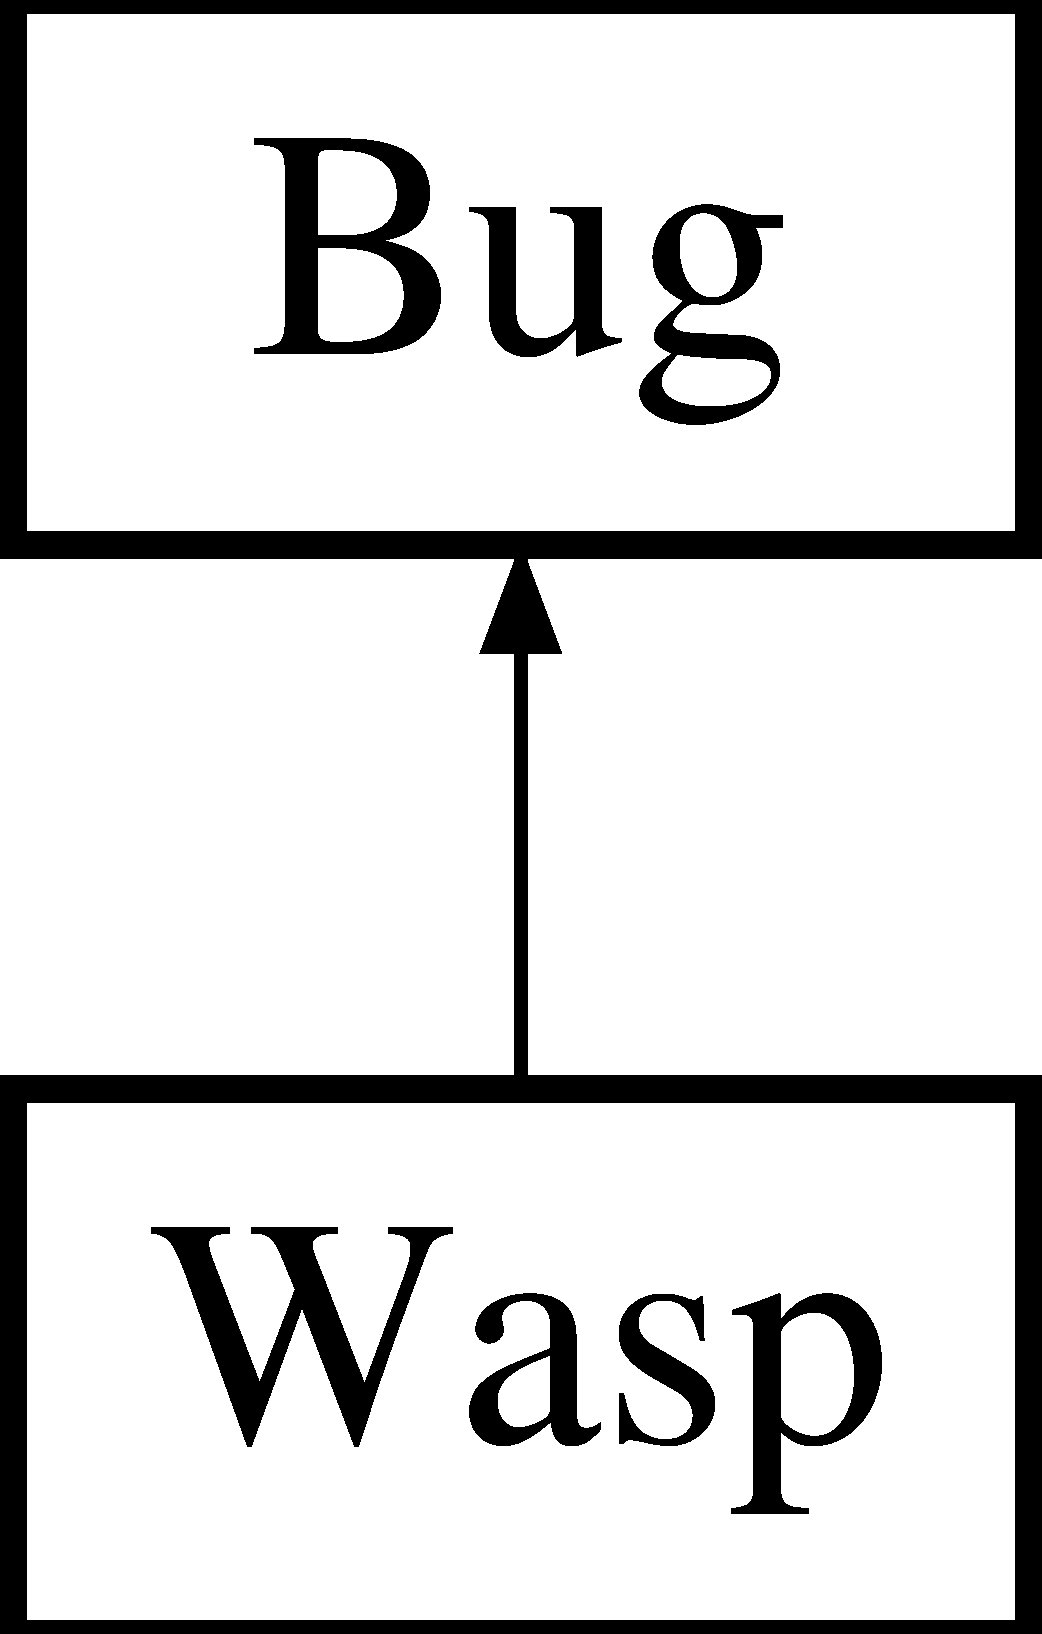
\includegraphics[height=2.000000cm]{classWasp}
\end{center}
\end{figure}
\subsection*{Signaux}
\begin{DoxyCompactItemize}
\item 
void \hyperlink{classBug_ab7379f5a0172e2d536e20f3f29915e02}{dead} (\hyperlink{classBug}{Bug} $\ast$bug)
\begin{DoxyCompactList}\small\item\em Signal de mort de l'insecte. \end{DoxyCompactList}\item 
void \hyperlink{classBug_a33f90dffa55e1dce80dc2416c75a53c8}{goalReached} (\hyperlink{classBug}{Bug} $\ast$bug)
\begin{DoxyCompactList}\small\item\em Signal d'arrivé. \end{DoxyCompactList}\end{DoxyCompactItemize}
\subsection*{Fonctions membres publiques}
\begin{DoxyCompactItemize}
\item 
\hypertarget{classWasp_a04c7736d744ab1c36b075f1e98ec93c2}{
{\bfseries Wasp} (double x, double y, double s, double start\_\-angle)}
\label{classWasp_a04c7736d744ab1c36b075f1e98ec93c2}

\item 
\hypertarget{classWasp_ac37833715ac95ea82a89c5cbd0fa26fb}{
void {\bfseries paint} (QPainter $\ast$painter, const QStyleOptionGraphicsItem $\ast$option, QWidget $\ast$widget)}
\label{classWasp_ac37833715ac95ea82a89c5cbd0fa26fb}

\item 
QRectF \hyperlink{classBug_a9b39c25361faad07b1bf2dd927d09dab}{boundingRect} () const 
\begin{DoxyCompactList}\small\item\em Surcharge de la fonction boudingRect() héritée de QGraphicsObject. \end{DoxyCompactList}\item 
QPainterPath \hyperlink{classBug_a587a36d3145c2b4dba6c689af22c65ac}{shape} () const 
\begin{DoxyCompactList}\small\item\em Surcharge de la méthode virtuelle pure \hyperlink{classBug_a587a36d3145c2b4dba6c689af22c65ac}{shape()} héritée de QGraphicsObject. \end{DoxyCompactList}\item 
void \hyperlink{classBug_a63402c05b5ba3fb034e41f1ced0e4b9f}{hit} (double dmg)
\begin{DoxyCompactList}\small\item\em Infliger des dégats à l'insecte. \end{DoxyCompactList}\item 
short int \hyperlink{classBug_aced471cedcfa855baddf4c827003e755}{getMoveType} ()
\begin{DoxyCompactList}\small\item\em Permet d'accéder à la valeur moveType de l'insecte. \end{DoxyCompactList}\end{DoxyCompactItemize}
\subsection*{Champs de données}
\begin{DoxyCompactItemize}
\item 
\hyperlink{classRender}{Render} $\ast$ \hyperlink{classBug_a7a93aae4e4b7a215c94ff85d0bd6e26d}{parent}
\begin{DoxyCompactList}\small\item\em L'objet \hyperlink{classRender}{Render} parent de l'insecte. \end{DoxyCompactList}\end{DoxyCompactItemize}
\subsection*{Fonctions membres protégées}
\begin{DoxyCompactItemize}
\item 
void \hyperlink{classBug_a8e0ea03e85c9324a13328da60e5c52ee}{advance} (int step)
\begin{DoxyCompactList}\small\item\em Implémentation de la fonction virtuelle pure \hyperlink{classBug_a8e0ea03e85c9324a13328da60e5c52ee}{advance()} héritée de QGGaphicsObject. \end{DoxyCompactList}\end{DoxyCompactItemize}
\subsection*{Attributs protégés}
\begin{DoxyCompactItemize}
\item 
double \hyperlink{classBug_a27a0f0b84d15525e409955509e6e3c42}{size}
\begin{DoxyCompactList}\small\item\em Taille. \end{DoxyCompactList}\item 
int \hyperlink{classBug_ad7e3597cf049f1051be94fcaf2fd3598}{frame}
\begin{DoxyCompactList}\small\item\em Compteur de frame. \end{DoxyCompactList}\item 
double \hyperlink{classBug_a13b95fbf23748ea853b01bfd0b0e7fc8}{speed}
\begin{DoxyCompactList}\small\item\em Vitesse de base. \end{DoxyCompactList}\end{DoxyCompactItemize}
\subsection*{Attributs privés}
\begin{DoxyCompactItemize}
\item 
\hypertarget{classWasp_abdd2e9eb377bb31907494f72067691f8}{
QImage $\ast$ {\bfseries image} \mbox{[}2\mbox{]}}
\label{classWasp_abdd2e9eb377bb31907494f72067691f8}

\end{DoxyCompactItemize}


\subsection{Documentation des fonctions membres}
\hypertarget{classBug_a8e0ea03e85c9324a13328da60e5c52ee}{
\index{Wasp@{Wasp}!advance@{advance}}
\index{advance@{advance}!Wasp@{Wasp}}
\subsubsection[{advance}]{\setlength{\rightskip}{0pt plus 5cm}void Bug::advance (
\begin{DoxyParamCaption}
\item[{int}]{step}
\end{DoxyParamCaption}
)\hspace{0.3cm}{\ttfamily  \mbox{[}protected, inherited\mbox{]}}}}
\label{classBug_a8e0ea03e85c9324a13328da60e5c52ee}
Implémentation de la fonction virtuelle pure \hyperlink{classBug_a8e0ea03e85c9324a13328da60e5c52ee}{advance()} héritée de QGGaphicsObject. 
\begin{DoxyParams}{Paramètres}
{\em step} & La fonction est appelé deux fois automatiquement par QT à chaque update(), une fois avec 0 comme paramètre puis une fois avec 1. \\
\hline
\end{DoxyParams}
\hypertarget{classBug_a9b39c25361faad07b1bf2dd927d09dab}{
\index{Wasp@{Wasp}!boundingRect@{boundingRect}}
\index{boundingRect@{boundingRect}!Wasp@{Wasp}}
\subsubsection[{boundingRect}]{\setlength{\rightskip}{0pt plus 5cm}QRectF Bug::boundingRect (
\begin{DoxyParamCaption}
{}
\end{DoxyParamCaption}
) const\hspace{0.3cm}{\ttfamily  \mbox{[}inherited\mbox{]}}}}
\label{classBug_a9b39c25361faad07b1bf2dd927d09dab}
Fonction appelé automatiquement par QT pour savoir s'il doit ou non réafficher l'insecte. \begin{DoxyReturn}{Renvoie}
Un objet QRectF correspondant au rectangle englobant l'ensemble du dessin de l'insecte. 
\end{DoxyReturn}
\hypertarget{classBug_ab7379f5a0172e2d536e20f3f29915e02}{
\index{Wasp@{Wasp}!dead@{dead}}
\index{dead@{dead}!Wasp@{Wasp}}
\subsubsection[{dead}]{\setlength{\rightskip}{0pt plus 5cm}void Bug::dead (
\begin{DoxyParamCaption}
\item[{{\bf Bug} $\ast$}]{bug}
\end{DoxyParamCaption}
)\hspace{0.3cm}{\ttfamily  \mbox{[}signal, inherited\mbox{]}}}}
\label{classBug_ab7379f5a0172e2d536e20f3f29915e02}
Signal émit lorsque l'insecte est tué. 
\begin{DoxyParams}{Paramètres}
{\em bug} & Un pointeur vers l'insecte qui vient de mourir. \\
\hline
\end{DoxyParams}
\hypertarget{classBug_aced471cedcfa855baddf4c827003e755}{
\index{Wasp@{Wasp}!getMoveType@{getMoveType}}
\index{getMoveType@{getMoveType}!Wasp@{Wasp}}
\subsubsection[{getMoveType}]{\setlength{\rightskip}{0pt plus 5cm}short int Bug::getMoveType (
\begin{DoxyParamCaption}
{}
\end{DoxyParamCaption}
)\hspace{0.3cm}{\ttfamily  \mbox{[}inherited\mbox{]}}}}
\label{classBug_aced471cedcfa855baddf4c827003e755}
\begin{DoxyReturn}{Renvoie}
la valeur prédéfinie FLY ou CRAWL. 
\end{DoxyReturn}
\hypertarget{classBug_a33f90dffa55e1dce80dc2416c75a53c8}{
\index{Wasp@{Wasp}!goalReached@{goalReached}}
\index{goalReached@{goalReached}!Wasp@{Wasp}}
\subsubsection[{goalReached}]{\setlength{\rightskip}{0pt plus 5cm}void Bug::goalReached (
\begin{DoxyParamCaption}
\item[{{\bf Bug} $\ast$}]{bug}
\end{DoxyParamCaption}
)\hspace{0.3cm}{\ttfamily  \mbox{[}signal, inherited\mbox{]}}}}
\label{classBug_a33f90dffa55e1dce80dc2416c75a53c8}
Signal émit par l'insecte lorsqu'il atteint son but. 
\begin{DoxyParams}{Paramètres}
{\em bug} & Un pointeur vers l'insecte. \\
\hline
\end{DoxyParams}
\hypertarget{classBug_a63402c05b5ba3fb034e41f1ced0e4b9f}{
\index{Wasp@{Wasp}!hit@{hit}}
\index{hit@{hit}!Wasp@{Wasp}}
\subsubsection[{hit}]{\setlength{\rightskip}{0pt plus 5cm}void Bug::hit (
\begin{DoxyParamCaption}
\item[{double}]{dmg}
\end{DoxyParamCaption}
)\hspace{0.3cm}{\ttfamily  \mbox{[}inherited\mbox{]}}}}
\label{classBug_a63402c05b5ba3fb034e41f1ced0e4b9f}
Fonction pouvant être appelée pour infliger des dégats à l'insecte (par exemple par les projectiles des tours). 
\begin{DoxyParams}{Paramètres}
{\em dmg} & Un double correspondant au point de dégat à infliger (avant réduction par la résistance de l'insecte). \\
\hline
\end{DoxyParams}


Réimplémentée dans \hyperlink{classAnt_a64b0e0e7d2605c1a5a0906587ab70920}{Ant}.

\hypertarget{classBug_a587a36d3145c2b4dba6c689af22c65ac}{
\index{Wasp@{Wasp}!shape@{shape}}
\index{shape@{shape}!Wasp@{Wasp}}
\subsubsection[{shape}]{\setlength{\rightskip}{0pt plus 5cm}QPainterPath Bug::shape (
\begin{DoxyParamCaption}
{}
\end{DoxyParamCaption}
) const\hspace{0.3cm}{\ttfamily  \mbox{[}inherited\mbox{]}}}}
\label{classBug_a587a36d3145c2b4dba6c689af22c65ac}
Fonction utilisé par QT pour traiter les collisions entre objets graphiques. \begin{DoxyReturn}{Renvoie}
Un object QPainterPath correspondant au contour de collision de l'insecte. 
\end{DoxyReturn}


\subsection{Documentation des champs}
\hypertarget{classBug_ad7e3597cf049f1051be94fcaf2fd3598}{
\index{Wasp@{Wasp}!frame@{frame}}
\index{frame@{frame}!Wasp@{Wasp}}
\subsubsection[{frame}]{\setlength{\rightskip}{0pt plus 5cm}int {\bf Bug::frame}\hspace{0.3cm}{\ttfamily  \mbox{[}protected, inherited\mbox{]}}}}
\label{classBug_ad7e3597cf049f1051be94fcaf2fd3598}
Compteur d'image utilisé pour afficher successivement chaque image des animations. \hypertarget{classBug_a7a93aae4e4b7a215c94ff85d0bd6e26d}{
\index{Wasp@{Wasp}!parent@{parent}}
\index{parent@{parent}!Wasp@{Wasp}}
\subsubsection[{parent}]{\setlength{\rightskip}{0pt plus 5cm}{\bf Render}$\ast$ {\bf Bug::parent}\hspace{0.3cm}{\ttfamily  \mbox{[}inherited\mbox{]}}}}
\label{classBug_a7a93aae4e4b7a215c94ff85d0bd6e26d}
Quand on ajoute un insecte à l'objet \hyperlink{classRender}{Render} par la méthode addBug(), cet attribut est automatiquement initialisé. \hypertarget{classBug_a27a0f0b84d15525e409955509e6e3c42}{
\index{Wasp@{Wasp}!size@{size}}
\index{size@{size}!Wasp@{Wasp}}
\subsubsection[{size}]{\setlength{\rightskip}{0pt plus 5cm}double {\bf Bug::size}\hspace{0.3cm}{\ttfamily  \mbox{[}protected, inherited\mbox{]}}}}
\label{classBug_a27a0f0b84d15525e409955509e6e3c42}
La taille de l'insecte, influe à la fois sur la taille de la représentation graphique et sur les caractéristiques de l'insecte.' \hypertarget{classBug_a13b95fbf23748ea853b01bfd0b0e7fc8}{
\index{Wasp@{Wasp}!speed@{speed}}
\index{speed@{speed}!Wasp@{Wasp}}
\subsubsection[{speed}]{\setlength{\rightskip}{0pt plus 5cm}double {\bf Bug::speed}\hspace{0.3cm}{\ttfamily  \mbox{[}protected, inherited\mbox{]}}}}
\label{classBug_a13b95fbf23748ea853b01bfd0b0e7fc8}
La vitesse en case/seconde à laquelle se déplace l'insecte. 

La documentation de cette classe a été générée à partir des fichiers suivants :\begin{DoxyCompactItemize}
\item 
src/Wasp.h\item 
src/Wasp.cpp\end{DoxyCompactItemize}

\hypertarget{classWater}{
\section{Référence de la classe Water}
\label{classWater}\index{Water@{Water}}
}
Graphe d'héritage de Water:\begin{figure}[H]
\begin{center}
\leavevmode
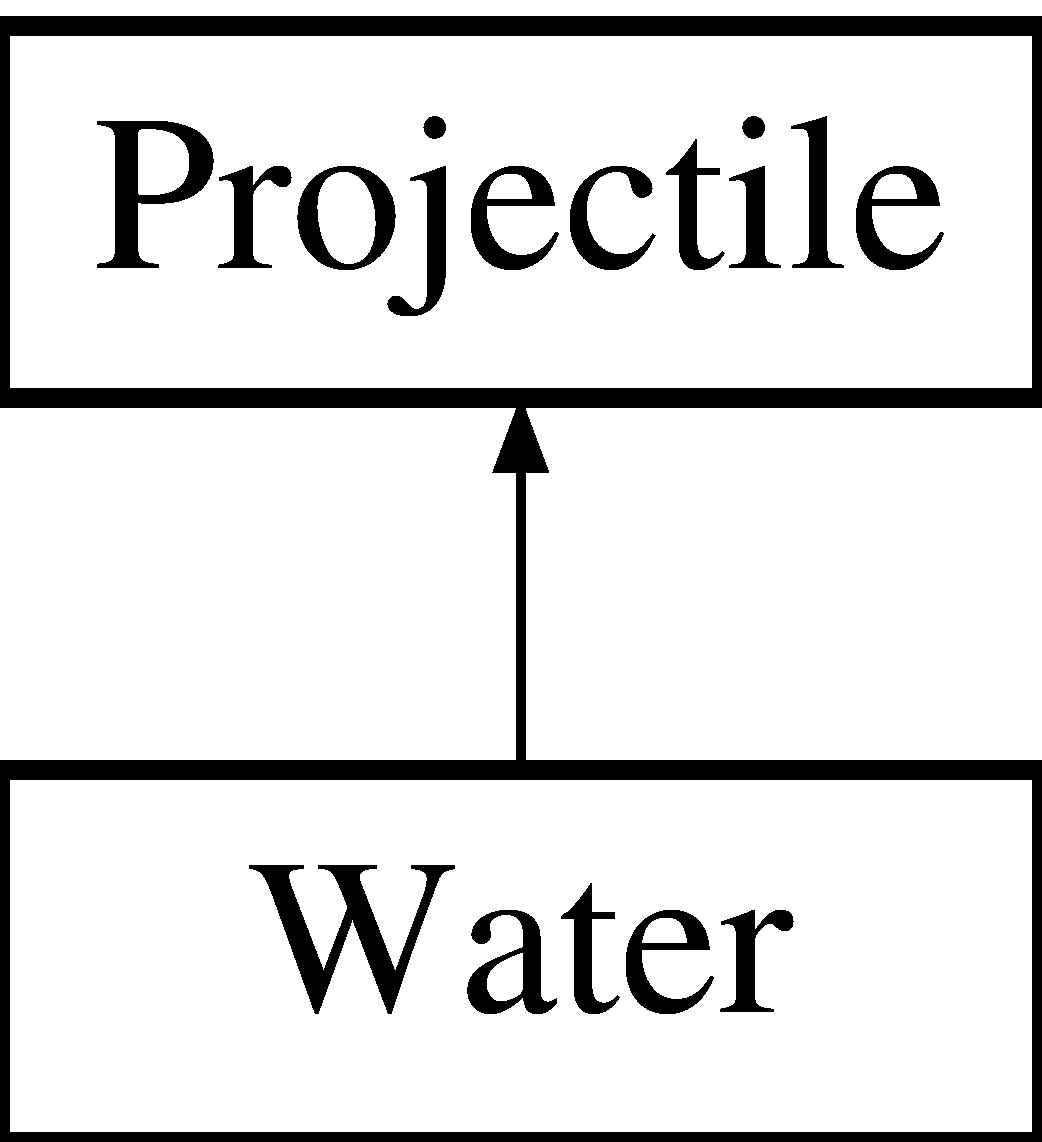
\includegraphics[height=2.000000cm]{classWater}
\end{center}
\end{figure}
\subsection*{Fonctions membres publiques}
\begin{DoxyCompactItemize}
\item 
\hypertarget{classWater_ada34e1066e8b672e509244a1bda18b48}{
{\bfseries Water} (QPointF start, QPointF dest, short int lvl)}
\label{classWater_ada34e1066e8b672e509244a1bda18b48}

\item 
\hypertarget{classWater_a1f8777c164bb06a357a78cabd9e790a2}{
void {\bfseries paint} (QPainter $\ast$painter, const QStyleOptionGraphicsItem $\ast$option, QWidget $\ast$widget)}
\label{classWater_a1f8777c164bb06a357a78cabd9e790a2}

\item 
\hypertarget{classProjectile_a0e0b18909c9c154404384707c6515802}{
QRectF {\bfseries boundingRect} () const }
\label{classProjectile_a0e0b18909c9c154404384707c6515802}

\item 
\hypertarget{classProjectile_aef0d6ffcea7620988cf5446d0c1133fa}{
void {\bfseries paint} (QPainter $\ast$painter, QColor color)}
\label{classProjectile_aef0d6ffcea7620988cf5446d0c1133fa}

\end{DoxyCompactItemize}
\subsection*{Fonctions membres protégées}
\begin{DoxyCompactItemize}
\item 
\hypertarget{classProjectile_a8e3b4bae49558a0febfce8c1accea72d}{
void {\bfseries advance} (int step)}
\label{classProjectile_a8e3b4bae49558a0febfce8c1accea72d}

\end{DoxyCompactItemize}


La documentation de cette classe a été générée à partir des fichiers suivants :\begin{DoxyCompactItemize}
\item 
src/Water.h\item 
src/Water.cpp\end{DoxyCompactItemize}

\printindex
\end{document}
